% !TEX encoding = UTF-8 Unicode
% !TEX TS-program = pdflatex

% toptesti document class
\documentclass[%
    a4paper, % not needed, by default it is a4paper, or also b5paper can be used
    corpo=13pt, % dimension of basic font
    % oneside is generally the way to go
    oneside, % two side optimizes for two-face printing, having chapters open on the right (aka odd numbers), if you don't want blank pages put oneside here
    stile=standard,
    %evenboxes, % not needed, to put supervisors and candidate at the same level
    tipotesi=magistrale,
    numerazioneromana, % roman numbering for appendixes and preambles, up to Table of Contents
    openright, % to force opening on the right for double-sided printing
    cucitura=7mm, % for printing, 7mm should be enough
    %dvipsnames, % for compatibility with xcolor, it does not work
]{toptesi}

\setlength{\parskip}{1em}

%%%%%%%%%%%%%%%%%%%%%%%%%%%%%%%%%%%%%%%%%%%%%%%%%%%%
\usepackage[english]{babel}
\usepackage[utf8]{inputenc}
\usepackage[T1]{fontenc}
\usepackage{lmodern}

\usepackage{hyperref} % must be loaded before glossaries-extra

% bibliography
\usepackage[hyperref=true,backref=false,backend=biber,maxbibnames=9,maxcitenames=2,style=numeric,citestyle=numeric,sorting=none]{biblatex} % hyperref uses links, backref goes back to citations, uses biber as backend, with 9 names at most in bibliography and 2 in citations, citing using numbers, and sorting in citation order
% sorting can be also ydnt for year descending, name, title or ynt for ascending year

\usepackage{adjustbox} % to resize boxes by keeping the same aspect ratio
\usepackage{algorithm} % algorithm environment
\usepackage{algpseudocode} % improved pseudo-code
\usepackage{amsfonts}               %  AMS mathematical fonts
\usepackage{amsmath}
\usepackage{amssymb}                %  AMS mathematical symbols
\usepackage{bm}                     %  black/bold mathematical symbols
\usepackage{booktabs}               %  better tables
\usepackage[labelfont=bf]{caption} % font=footnotesize % to have reduced caption font size
\usepackage{csquotes}
\usepackage{enumitem} %left align the bulleted points
\usepackage{geometry}
%\usepackage{glossaries} % to use acronyms and glossary, it has also glossaries-extra as extension, but commands are different
\usepackage[%
    toc, % puts the link in the ToC
    %record, % to use bib2gls
    abbreviations, % to load abbreviations / acronyms
    nonumberlist, % to avoid printing the numbers of the references in the acronyms page
]{glossaries-extra}
\usepackage{graphicx}               %  post-script images
%\usepackage{iwona} % extra fonts, substitute standard ones
\usepackage{listings} % to insert formatted code
\usepackage{lipsum} % for lorem ipsum text, not needed in the real work
\usepackage{makecell} % to change dimensions of cells, for math cases
\usepackage{mathtools} % for additional commands
\usepackage{mfirstuc} % to have capitalization capabilities
\usepackage[final]{microtype}      % microtypography, final lets latex use it also in bibliography
\usepackage{multirow} % to allow for cells covering more than 1 row in tables
\usepackage{nicefrac}       % compact symbols for 1/2, etc.
%\usepackage[lofdepth,lotdepth]{subfig}
\usepackage{ragged2e} % for justifying text
\usepackage{siunitx} % support for SI units of measurement and number typesetting
\usepackage{subfig}
\usepackage{svg} % for svg support, works only if inkscape is installed, default for Overleaf v2
%\usepackage{subfigure}              %  subfigure compatibility, can be removed if subfig
\usepackage{tabularx} % equal-width columns in tables
\usepackage{textcomp} % extra fonts and symbols
\usepackage{url}            % simple URL typesetting
\usepackage{verbatim} % for extended verbatim support
\usepackage{xcolor} % to define colors and use standard CSS names add dvipsnames as option, but it clashes with xcolor loaded in toptesi, pay attention that if it goes in conflict with tikz/beamer, simply use \documentclass[usenames,dvipsnames]{beamer}, along with other custom options when defining the document class

% MY PACKAGES
\usepackage{changepage}
\usepackage{todonotes}


% configuration for glossaries
% convert and load converted glossaries in .tex ,format from .bib
\setabbreviationstyle{long-short-desc} % style before loading resources
% this command sets the style to title for long names of acronyms only in the glossary description, leading to capitalized first-letter for all words
% \glssetcategoryattribute{\glsxtrabbrvtype}{glossname}{capitalisewords} % doesn't work
% resources to load if using a bib file with bib2gls
%\GlsXtrLoadResources[%
% src={glossaries}, % name of the file without extension
% selection=all, % select all the entries
%]
% not needed
%\newglossary*{abbreviation}{Acronyms} % to change the name of this glossary for acronyms

%\renewcommand{\glsclearpage}{\paginavuota} % to allow glossaries to clear pages, done manually is better


% setup for hyperref
\hypersetup{%
    pdfpagemode={UseOutlines},
    bookmarksopen,
    pdfstartview={FitH},
    colorlinks,
    linkcolor={black}, % it is suggested to keep them black, since when printing it it costs per page, and if they have color it's twice the price per page
    citecolor={black},
    urlcolor={black}
  }
%

% setup for svg
\svgsetup{%
    inkscapeformat=pdf, % to force usage of PDF
    inkscapelatex=false, % to disable latex rendering of text, produces errors
}

% setup for siunitx, it does not work in the summary
\sisetup{%
    detect-all, % to use the same font as for writing when using \num
    mode=text, % to allow it to work also in math mode
    group-separator = {,}, % separator for number grouping
    group-minimum-digits = 3, % minimum number of digits a number must have to be grouped in 3-digit groups
}

% listings colours
\definecolor{rulecolor}{rgb}{0,0,0}
\definecolor{commentcolor}{rgb}{0,0.6,0}
\definecolor{linenumbercolor}{rgb}{0.5,0.5,0.5}
\definecolor{keywordcolor}{rgb}{0,0,0.95}
\definecolor{backcolor}{rgb}{1,1,1}%{0.95,0.95,0.92}
\definecolor{stringcolor}{rgb}{0.58,0,0.82}

% setup for lstlisting
\lstset{ %
    aboveskip=5mm,
	backgroundcolor=\color{backcolor},   % choose the background color; you must add \usepackage{color} or \usepackage{xcolor}; should come as last argument
	basicstyle=\footnotesize\ttfamily,        % the size of the fonts that are used for the code
	breakatwhitespace=false,         % sets if automatic breaks should only happen at whitespace
	breaklines=true,                 % sets automatic line breaking
	captionpos=t,                    % sets the caption-position to bottom
	commentstyle=\color{commentcolor},    % comment style
	extendedchars=true,              % lets you use non-ASCII characters; for 8-bits encodings only, does not work with UTF-8
	frame=single,	                   % adds a frame around the code
	keepspaces=true,                 % keeps spaces in text, useful for keeping indentation of code (possibly needs columns=flexible)
	keywordstyle=\color{keywordcolor},       % keyword style
	%language=VHDL,                 % the language of the code
	numbers=left,                    % where to put the line-numbers; possible values are (none, left, right)
	numbersep=5pt,                   % how far the line-numbers are from the code
	numberstyle=\tiny\color{linenumbercolor}, % the style that is used for the line-numbers
	rulecolor=\color{rulecolor},         % if not set, the frame-color may be changed on line-breaks within not-black text (e.g. comments (green here))
	showspaces=false,                % show spaces everywhere adding particular underscores; it overrides 'showstringspaces'
	showstringspaces=false,          % underline spaces within strings only
	showtabs=false,                  % show tabs within strings adding particular underscores
	stepnumber=1,                    % the step between two line-numbers. If it's 1, each line will be numbered
	stringstyle=\color{stringcolor},     % string literal style
	tabsize=4,	                   % sets default tabsize to 2 spaces
	title=\lstname,                   % show the filename of files included with \lstinputlisting; also try caption instead of title
	inputencoding=utf8,
	literate=
	{á}{{\'a}}1 {é}{{\'e}}1 {í}{{\'i}}1 {ó}{{\'o}}1 {ú}{{\'u}}1
	{Á}{{\'A}}1 {É}{{\'E}}1 {Í}{{\'I}}1 {Ó}{{\'O}}1 {Ú}{{\'U}}1
	{à}{{\`a}}1 {è}{{\`e}}1 {ì}{{\`i}}1 {ò}{{\`o}}1 {ù}{{\`u}}1
	{À}{{\`A}}1 {È}{{\'E}}1 {Ì}{{\`I}}1 {Ò}{{\`O}}1 {Ù}{{\`U}}1
	{ä}{{\"a}}1 {ë}{{\"e}}1 {ï}{{\"i}}1 {ö}{{\"o}}1 {ü}{{\"u}}1
	{Ä}{{\"A}}1 {Ë}{{\"E}}1 {Ï}{{\"I}}1 {Ö}{{\"O}}1 {Ü}{{\"U}}1
	{â}{{\^a}}1 {ê}{{\^e}}1 {î}{{\^i}}1 {ô}{{\^o}}1 {û}{{\^u}}1
	{Â}{{\^A}}1 {Ê}{{\^E}}1 {Î}{{\^I}}1 {Ô}{{\^O}}1 {Û}{{\^U}}1
	{œ}{{\oe}}1 {Œ}{{\OE}}1 {æ}{{\ae}}1 {Æ}{{\AE}}1 {ß}{{\ss}}1
	{ű}{{\H{u}}}1 {Ű}{{\H{U}}}1 {ő}{{\H{o}}}1 {Ő}{{\H{O}}}1
	{ç}{{\c c}}1 {Ç}{{\c C}}1 {ø}{{\o}}1 {å}{{\r a}}1 {Å}{{\r A}}1
	{€}{{\euro}}1 {£}{{\pounds}}1 {«}{{\guillemotleft}}1
	{»}{{\guillemotright}}1 {ñ}{{\~n}}1 {Ñ}{{\~N}}1 {¿}{{?`}}1
}


% biblatex setup
% generally 9000 is ok, if higher than 10000 it's bad
% If you want to break on URL numbers
\setcounter{biburlnumpenalty}{9000}
% If you want to break on URL lower case letters
\setcounter{biburllcpenalty}{9000}
% If you want to break on URL UPPER CASE letters
\setcounter{biburlucpenalty}{9000}



% how to change Contents to Table of Contents
\addto\captionsenglish{% Replace "english" with the language you use
  \renewcommand{\contentsname}%
    {Table of Contents}%
}

% to change the name of Abbreviations to Acronyms
% not needed if use use entry types and define those
% \renewcommand{\abbreviationsname}{Acronyms}

% to allow line comments in algorithms
\algnewcommand{\LineComment}[1]{\State \(\triangleright\) #1}

% to declare abs and norm
\DeclarePairedDelimiter\abs{\lvert}{\rvert}%
\DeclarePairedDelimiter\norm{\lVert}{\rVert}%

% Swap the definition of \abs* and \norm*, so that \abs
% and \norm resizes the size of the brackets, and the 
% starred version does not.
\makeatletter
\let\oldabs\abs
\def\abs{\@ifstar{\oldabs}{\oldabs*}}
%
\let\oldnorm\norm
\def\norm{\@ifstar{\oldnorm}{\oldnorm*}}
\makeatother


% change this configuration with your info
% if you need fewer or more supervisors you have to change \relatore command by adding or removing lines in the table in toptesi_config
\newcommand{\thesistitle}{Title of this thesis}
\newcommand{\thesisuniversitylogo}{images/logo/polito_eurecom_logo.png} % choose your logo
\newcommand{\thesiscandidatename}{Gabriele}
\newcommand{\thesiscandidatesurname}{Gioetto}
\newcommand{\thesissupervisoronetitle}{dr.}
\newcommand{\thesissupervisoronename}{Francesco}
\newcommand{\thesissupervisoronesurname}{Di Cerbo}
\newcommand{\thesissupervisortwotitle}{prof.}
\newcommand{\thesissupervisortwoname}{Paolo}
\newcommand{\thesissupervisortwosurname}{Papotti}
\newcommand{\thesissupervisorthreetitle}{prof.}
\newcommand{\thesissupervisorthreename}{Giuseppe}
\newcommand{\thesissupervisorthreesurname}{Rizzo}
\newcommand{\thesisdate}{Academic Year 2022/2023 \\ Torino}
\newcommand{\thesiscourse}{Data Science and Engineering}
\newcommand{\thesisuniversity}{Politecnico di Torino}
\newcommand{\thesislevel}{Master} % master or bachelor
\newcommand{\thesiscandidatetext}{Candidate:}
\newcommand{\thesissupervisortext}{Supervisors:}


% fontsize is {size}{spacing}\family
\newcommand {\institutionfont}{\fontsize {22}{30}\scshape}
\newcommand {\divisionfont}{\fontsize {16}{20}\rmfamily}
\newcommand {\pretitlefont}{\fontsize {16}{16}\rmfamily}
\newcommand {\customtitlefont}{\fontsize {21}{28}\scshape}% {iwona}{bx}{n}}
\newcommand {\fixednamesfont}{\fontsize {16}{20}\mdseries}
\newcommand {\namesfont}{\fontsize {15}{20}\bfseries}
\newcommand {\footfont}{\fontsize {15}{18}\rmfamily}


\addbibresource{biblio.bib}


\begin{document}

\overfullrule=0.00001pt % latex shows a black bar for overfulls over this dimension

%\emergencystretch=1em % to allow some stretching in the lines to avoid overfull boxes, also in bibliography, eventually can be used only before bibliography or in the preamble for the whole document, not needed if using biblatex configuration in most cases


\ateneo{\thesisuniversity} % university name
\logosede[5cm]{\thesisuniversitylogo} % logo, square brackets contain the height

\titolo{\thesistitle} % title
%\sottotitolo{Metodo dei satelliti medicei} % subtitle

% place/remove a slash \\ to put the name on the following line or after Master Degree Course
\corsodilaurea{\thesiscourse} % course name


%~251197 % id number is not needed

\candidato{\thesiscandidatename~\textsc{\thesiscandidatesurname}} % candidate

% using tabular we can have more than 1 supervisor under the same column
\relatore{\tabular{@{}l}%
    \xmakefirstuc{\thesissupervisoronetitle}~\thesissupervisoronename~\textsc{\thesissupervisoronesurname}\\[0.4ex]
    \xmakefirstuc{\thesissupervisortwotitle}~\thesissupervisortwoname~\textsc{\thesissupervisortwosurname}\\[0.4ex]
    \xmakefirstuc{\thesissupervisorthreetitle}~\thesissupervisorthreename~\textsc{\thesissupervisorthreesurname}\\[0.4ex]
    \endtabular}

% in this way we have Academic Year without stile=classica, so without lines
%\sedutadilaurea{\textsc{Academic~Year} 2019-2020}% per la laurea magistrale
% for PoliTo there is only month year
\sedutadilaurea{\thesisdate}% per la laurea magistrale
% PhD
%\esamedidottorato{Novembre 1610}
%\ciclodidottorato{XV}

% offset for binding, the smaller the better
%\setbindingcorrection{3mm}


\english% or \italian (default)

\iflanguage{english}{%
	%\retrofrontespizio{This work is subject to the Creative Commons Licence}

	\CorsoDiLaureaIn{\thesislevel's Degree Course in\space}

	\TesiDiLaurea{\thesislevel's Degree Thesis}

	\InName{in}
	\CandidateName{\xmakefirstuc{\thesiscandidatetext}}% or Candidates
	\AdvisorName{\xmakefirstuc{\thesissupervisortext}}% or Supervisor
	%\TutorName{Tutor}
	%\NomeTutoreAziendale{Internship Tutor}

	%\NomePrimoTomo{First volume}
	%\NomeSecondoTomo{Second Volume}
	%\NomeTerzoTomo{Third Volume}
	%\NomeQuartoTomo{Fourth Volume}
}{}


% front page
% frontespizio can be used for the first page print
% while the custom-made frontpage can be used as hard-cover
% use pdfjoin or pdfseparate to extract or put together the pages if needed
%\frontespizio* % without star the logo is on top
\newgeometry{top=2cm,left=3cm,right=3cm,bottom=2cm,heightrounded}
\begin{titlepage}
\centering
%
{\institutionfont \textbf{\MakeUppercase{\thesisuniversity}} \par}
%
\vspace{\stretch{2}} % changing this number and the others changes the proportion
%
{\divisionfont \textbf{\thesislevel's Degree in \thesiscourse} \par}
%
\vspace{\stretch{3}}
%
\includegraphics[width=70mm]{\thesisuniversitylogo}\\
%
\vspace{\stretch{4}}
%
{\divisionfont \textbf{\thesislevel's Degree Thesis} \par}
%
\vspace{\stretch{3}}
%
{\customtitlefont \textbf{\thesistitle} \par}
%
\vspace{\stretch{10}}
%
\makebox[\textwidth]{\null\hfill\def\arraystretch{2}% % to change the spacing change this number
\begin{minipage}[t]{.5\textwidth}\raggedright
    \begin{tabular}[t]{@{}l@{}}
        \fixednamesfont \textbf{\thesissupervisortext} \\
        \namesfont \xmakefirstuc{\thesissupervisoronetitle}~\thesissupervisoronename~\thesissupervisoronesurname\\
        \namesfont \xmakefirstuc{\thesissupervisortwotitle}~\thesissupervisortwoname~\thesissupervisortwosurname\\
    \end{tabular}
\end{minipage}
%
\hfill
%
\begin{minipage}[t]{.5\textwidth}\raggedleft
    \begin{tabular}[t]{@{}r@{}}
        \fixednamesfont \textbf{\thesiscandidatetext} \\
        \namesfont \thesiscandidatename~\thesiscandidatesurname
    \end{tabular}
\end{minipage}\hfill\null}\\
%
\vspace{\stretch{5}}
%
{\footfont \textbf{\thesisdate} \par}
%
\end{titlepage}

\restoregeometry
 % custom frontpage
%\retrofrontespizio
% insert text for the back of the front page
% if you insert any remove the following \paginavuota
% either a blank page or a back is needed to have double-sided printing
% pay attention to leave the space for the page

%\paginavuota % clears a page

\frontmatter

% abstract if needed
% \begin{abstract}
%     \chapter*{Abstract}

An HR (Human Resources) department in a large organization receives inquiries\slash requests from employees on multiple topics, which are quite different from one another. As an example, an employee can send requests dealing with health conditions, compensation/taxation, events of life (marriage, death of a relative\dots)\dots. \\
These data can be used for many different queries that can be useful for analysis purposes (Example: `How many people have had COVID during 2021`). However, HR tickets typically contain personal data, that cannot be processed without the consent of the data subject according to the European privacy regulation (GDPR). \\
To be able to process documents with personal data, we can identify the pieces of information that qualify as personal data in a communication and subsequently anonymize such information using the appropriate techniques.
A significant part of this problem is represented by the complex nature of personal data according to GDPR:\@ personal data are defined as `\textit{any piece of information that can be connected to an identified or identifiable natural person}` It comprises obvious identifiers like social security numbers, email addresses but also, elements like `the Italian intern working for SAP in South of France`.
To the best of our knowledge, it does not exist a public dataset of HR tickets which can be used to train machine learning models, the main reason being the difficult nature of these types of data. Synthetic data, which are artificial data that are generated from original data and a model that is trained to reproduce the characteristics and structure of the original data, follow a data protection by design approach.
To address the need for a large dataset of HR tickets, we created a taxonomy of tickets, we found real data that can be used as support to create synthetic tickets and developed Ticket Generator: an application that can produce as many tickets as needed belonging to different categories, we released a dataset of previously created tickets and we showcase some possible use cases of the dataset.

% \end{abstract}

% to create blank pages for openright in frontmatter
% use one of the following two methods
% 1) use the following three lines
%\phantom{0} % needed otherwise cleardoublepage does not clean the page because it sees it empty
%\cleardoublepage
%\thispagestyle{empty} % to have empty page, without numbers
% 2) or
\paginavuota % to manually create a blank page

\chapter*{Abstract}

An HR (Human Resources) department in a large organization receives inquiries\slash requests from employees on multiple topics, which are quite different from one another. As an example, an employee can send requests dealing with health conditions, compensation/taxation, events of life (marriage, death of a relative\dots)\dots. \\
These data can be used for many different queries that can be useful for analysis purposes (Example: `How many people have had COVID during 2021`). However, HR tickets typically contain personal data, that cannot be processed without the consent of the data subject according to the European privacy regulation (GDPR). \\
To be able to process documents with personal data, we can identify the pieces of information that qualify as personal data in a communication and subsequently anonymize such information using the appropriate techniques.
A significant part of this problem is represented by the complex nature of personal data according to GDPR:\@ personal data are defined as `\textit{any piece of information that can be connected to an identified or identifiable natural person}` It comprises obvious identifiers like social security numbers, email addresses but also, elements like `the Italian intern working for SAP in South of France`.
To the best of our knowledge, it does not exist a public dataset of HR tickets which can be used to train machine learning models, the main reason being the difficult nature of these types of data. Synthetic data, which are artificial data that are generated from original data and a model that is trained to reproduce the characteristics and structure of the original data, follow a data protection by design approach.
To address the need for a large dataset of HR tickets, we created a taxonomy of tickets, we found real data that can be used as support to create synthetic tickets and developed Ticket Generator: an application that can produce as many tickets as needed belonging to different categories, we released a dataset of previously created tickets and we showcase some possible use cases of the dataset.


\chapter*{Acknowledgements}



\chapter*{About SAP}

Founded in 1972, SAP has grown to become the world's leading provider of business software solutions. SAP is market leader in enterprise application software. The company is also the fastest-growing major database company. Globally, more than 77\% of all business transactions worldwide touch an SAP software system.

With more than 347.000 customers in more than 180 countries, SAP includes subsidiaries in all major countries. SAP is the world's largest inter-enterprise software company and the world's third-largest independent software supplier, overall. SAP solutions help enterprises of all sizes around the world to improve customer relationships, enhance partner collaboration and create efficiencies across their supply chains and business operations. SAP employs more than 98.600 people.

\section*{Security Research at SAP Labs France, Sophia Antipolis} 

Based at SAP Labs France Mougins, Security Research Sophia-Antipolis\cite{sap} addresses the upcoming security needs, focusing on increased automation of the security life cycle and on providing innovative solutions for the security challenges in networked businesses, including cloud, services and mobile. This internship is based in the SAP Labs France Research Lab, in Sophia-Antipolis. The work will be performed in the context of the Research Program "Security {\&} Trust".

\paginavuota
\tableofcontents

\listoffigures % ToC for figures

% actually abbreviation is the name used for acronym in glossaries-extra
% title sets the name
% type tells the type of glossary to print
% style overrides the global style
% here we are printing only abbreviations
% printunsrtglossary if using record, otherwise printglossary is ok
\paginavuota
\printunsrtglossary[style=altlist,title=Acronyms,type=\glsxtrabbrvtype]

% also list of symbols here if needed

% to remove all first use occurrences given the presence of the summary
\glsresetall
% to skip all the first use occurrences, using only short forms
% \glsunsetall


\mainmatter

%\part{Prima Parte} % parts division, not needed
% Chapters always open on a right-side page, i.e. odd numbers, so a blank page is inserted if needed
%\cleardoublepage[empty] % to have a fully blank page
% a blank page appears before the first chapter in some configurations, on the last version it doesn't

% list here all the chapters
\chapter{Introduction}
\label{sec:Introduction}


With the advent of deep learning, a lot of applications have been needing more and more data. However, more often than not, these data contain a large amount of sensitive and personal information that restricts its use according to the legal framework in place in many countries. \\
Data is growing rapidly within companies, containing a great deal of sensitive information that can't be processed or shared without due consideration of legal ramifications. If such data could reveal the identity of someone, their personal rights would be threatened. \\
This is especially relevant in the context of HR tickets, which can contain not only personal information but also special categories of personal data, which require extra protection according to GDPR. \\


\section{GDPR}
The General Data Protection Regulation is a privacy regulation that regulates the processing of personal data \textit{"wholly or partly by automated means and to the processing other than by automated means"}. The regulation applies to all citizens of the EU and to all data subjects in the EU, whether the processing is carried out inside or outside the EU. \\
Personal data are defined as \textit{"any information relating to an identified or identifiable natural person"}. The regulation states that \textit{"an identifiable natural person is one who can be identified, directly or indirectly, in particular by reference to an identifier such as a name, an identification number, location data, an online identifier or to one or more factors specific to the physical, physiological, genetic, mental, economic, cultural or social identity of that natural person"}. The natural person can be identified both by direct identifiers and quasi-identifiers. The direct identifiers are information that directly identify the person, such as the telephone number, social security number\dots, while the quasi-identifiers are information that alone cannot identify a person, but if they are combined with other quasi-identifiers can affect a person's privacy. For example, the job title could be not enough to identify a person, but combined with his/her company and his/her nationality it could be. \\
Moreover, the GDPR treats some categories of personal data more carefully. These categories are called 'special categories' and include racial or ethnic origin, political opinions, religious or philosophical beliefs, trade union membership, genetic data, biometric data, data concerning health or data concerning a natural person's sex life or sexual orientation \\
The special categories of personal data cannot be generally processed, with some exceptions including "the data subject has given explicit consent to the processing of those personal data for one or more specified purposes".\\


\section{Synthetic data}
Synthetic data is artificial data that is generated from real data and has the same statistical distribution as the original data. This means that synthetic data and original data should deliver very similar results when undergoing the same statistical analysis. \\
Synthetic data has many benefits over real data: if you create a model that generates synthetic data you can generate how many data you need, you can infer certain properties to your data ( for example it can be useful for bias and fairness research ) and above all, synthetic data can respect the right to personal data protection. It is important to point out that it is not always guaranteed that synthetic data is privacy-preserving: it has been shown that synthetic data can leak personal information \cite{bellovin2019privacy}.\\

\section{Ticket Generation}
We created a tool that can be used to create an unlimited amount of synthetic HR tickets and we published a dataset of 16000 tickets. Each ticket, other than the ticket's text, is composed of a category, sub-category and the entities of the ticket. The tickets are not created from scratch, but starting from real-world's datasets and some prompts that help the model generate the text. \\
We did a survey internal to the company to gather some real data, and we changed the ticket generation parameters in order to respect the real data with respect to different text metrics. \\
Finally, we showed different possible use cases for the dataset:
\begin{itemize}
    \item Ticket Anonymization
    \item Ticket Classification
    \item Named Entity Recognition on tickets' entities
\end{itemize}
\chapter{Related Works}
\label{sec:RelatedWorks}

Due to the sensitive nature of the data and GDPR laws, a dataset of HR tickets written by company employees has never been published as far as we know. This is likely to be the case because it could be damaging for both the company and the employees, such as an employee criticizing the working environment or revealing company's confidential information in a ticket.  \\
However, some datasets can resemble what we are trying to build, with similar language style and intents:
\begin{itemize}
    \item \textit{Consumer Complaint}: Consumer Financial Protection Bureau's online database of customer complaints about different financial products. The overall dataset contains over 600,000 complaints and each record has the complaint's text description, the product that is the cause of the complaint, the company which issues the product, and the category of the issue. In the dataset the personal information are masked.
    \item \textit{Enron Mail}: The \textit{Enron Mail} dataset contains about 0.5M emails of 150 senior management from the Enron corporation. This data was originally made public, and posted to the web, by the Federal Energy Regulatory Commission during its investigation for fraud. The corpus is one of the only few publicly available mass collections of real emails easily available for study.
    \item \textit{TAB}: the Text Anonymization Benchmark corpus\cite{pilan2022text} is a privacy-oriented annotated text resource. The corpus comprises 1,268 English-language court cases from the European Court of Human Rights (ECHR) enriched with comprehensive annotations about the personal information appearing in each document, including their semantic category, identifier type, confidential
    attributes, and co-reference relations.
\end{itemize}


\chapter{Method}
\label{sec:Method}


\section{Taxonomy}

\begin{figure}[h] 
    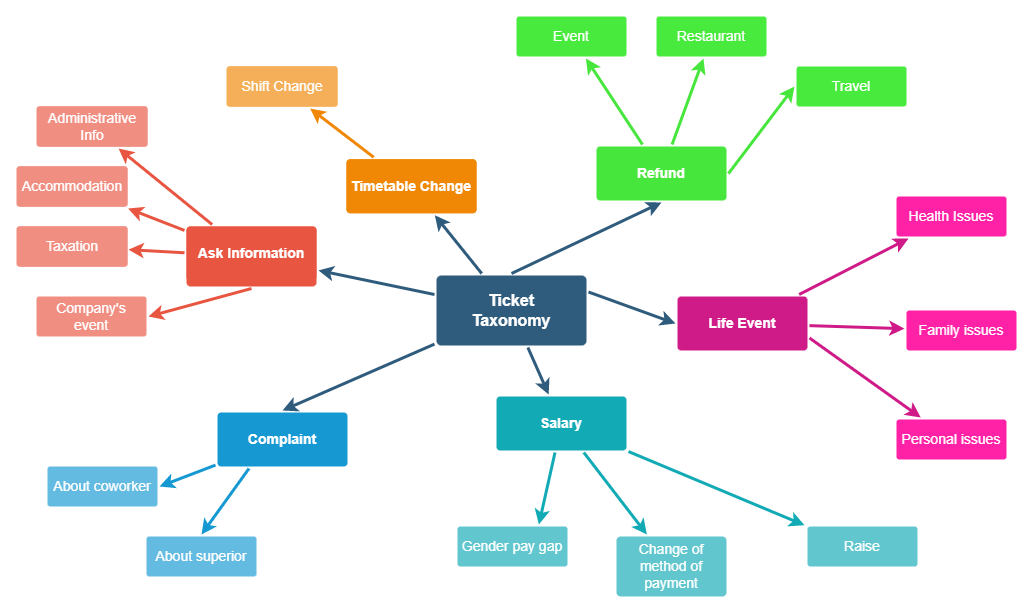
\includegraphics[width=\textwidth]{images/Taxonomy_Tickets.drawio.png}
    \caption{Initial Taxonomy}
    \label{fig:taxonomy}
\end{figure}    

\begin{figure}[h] 
    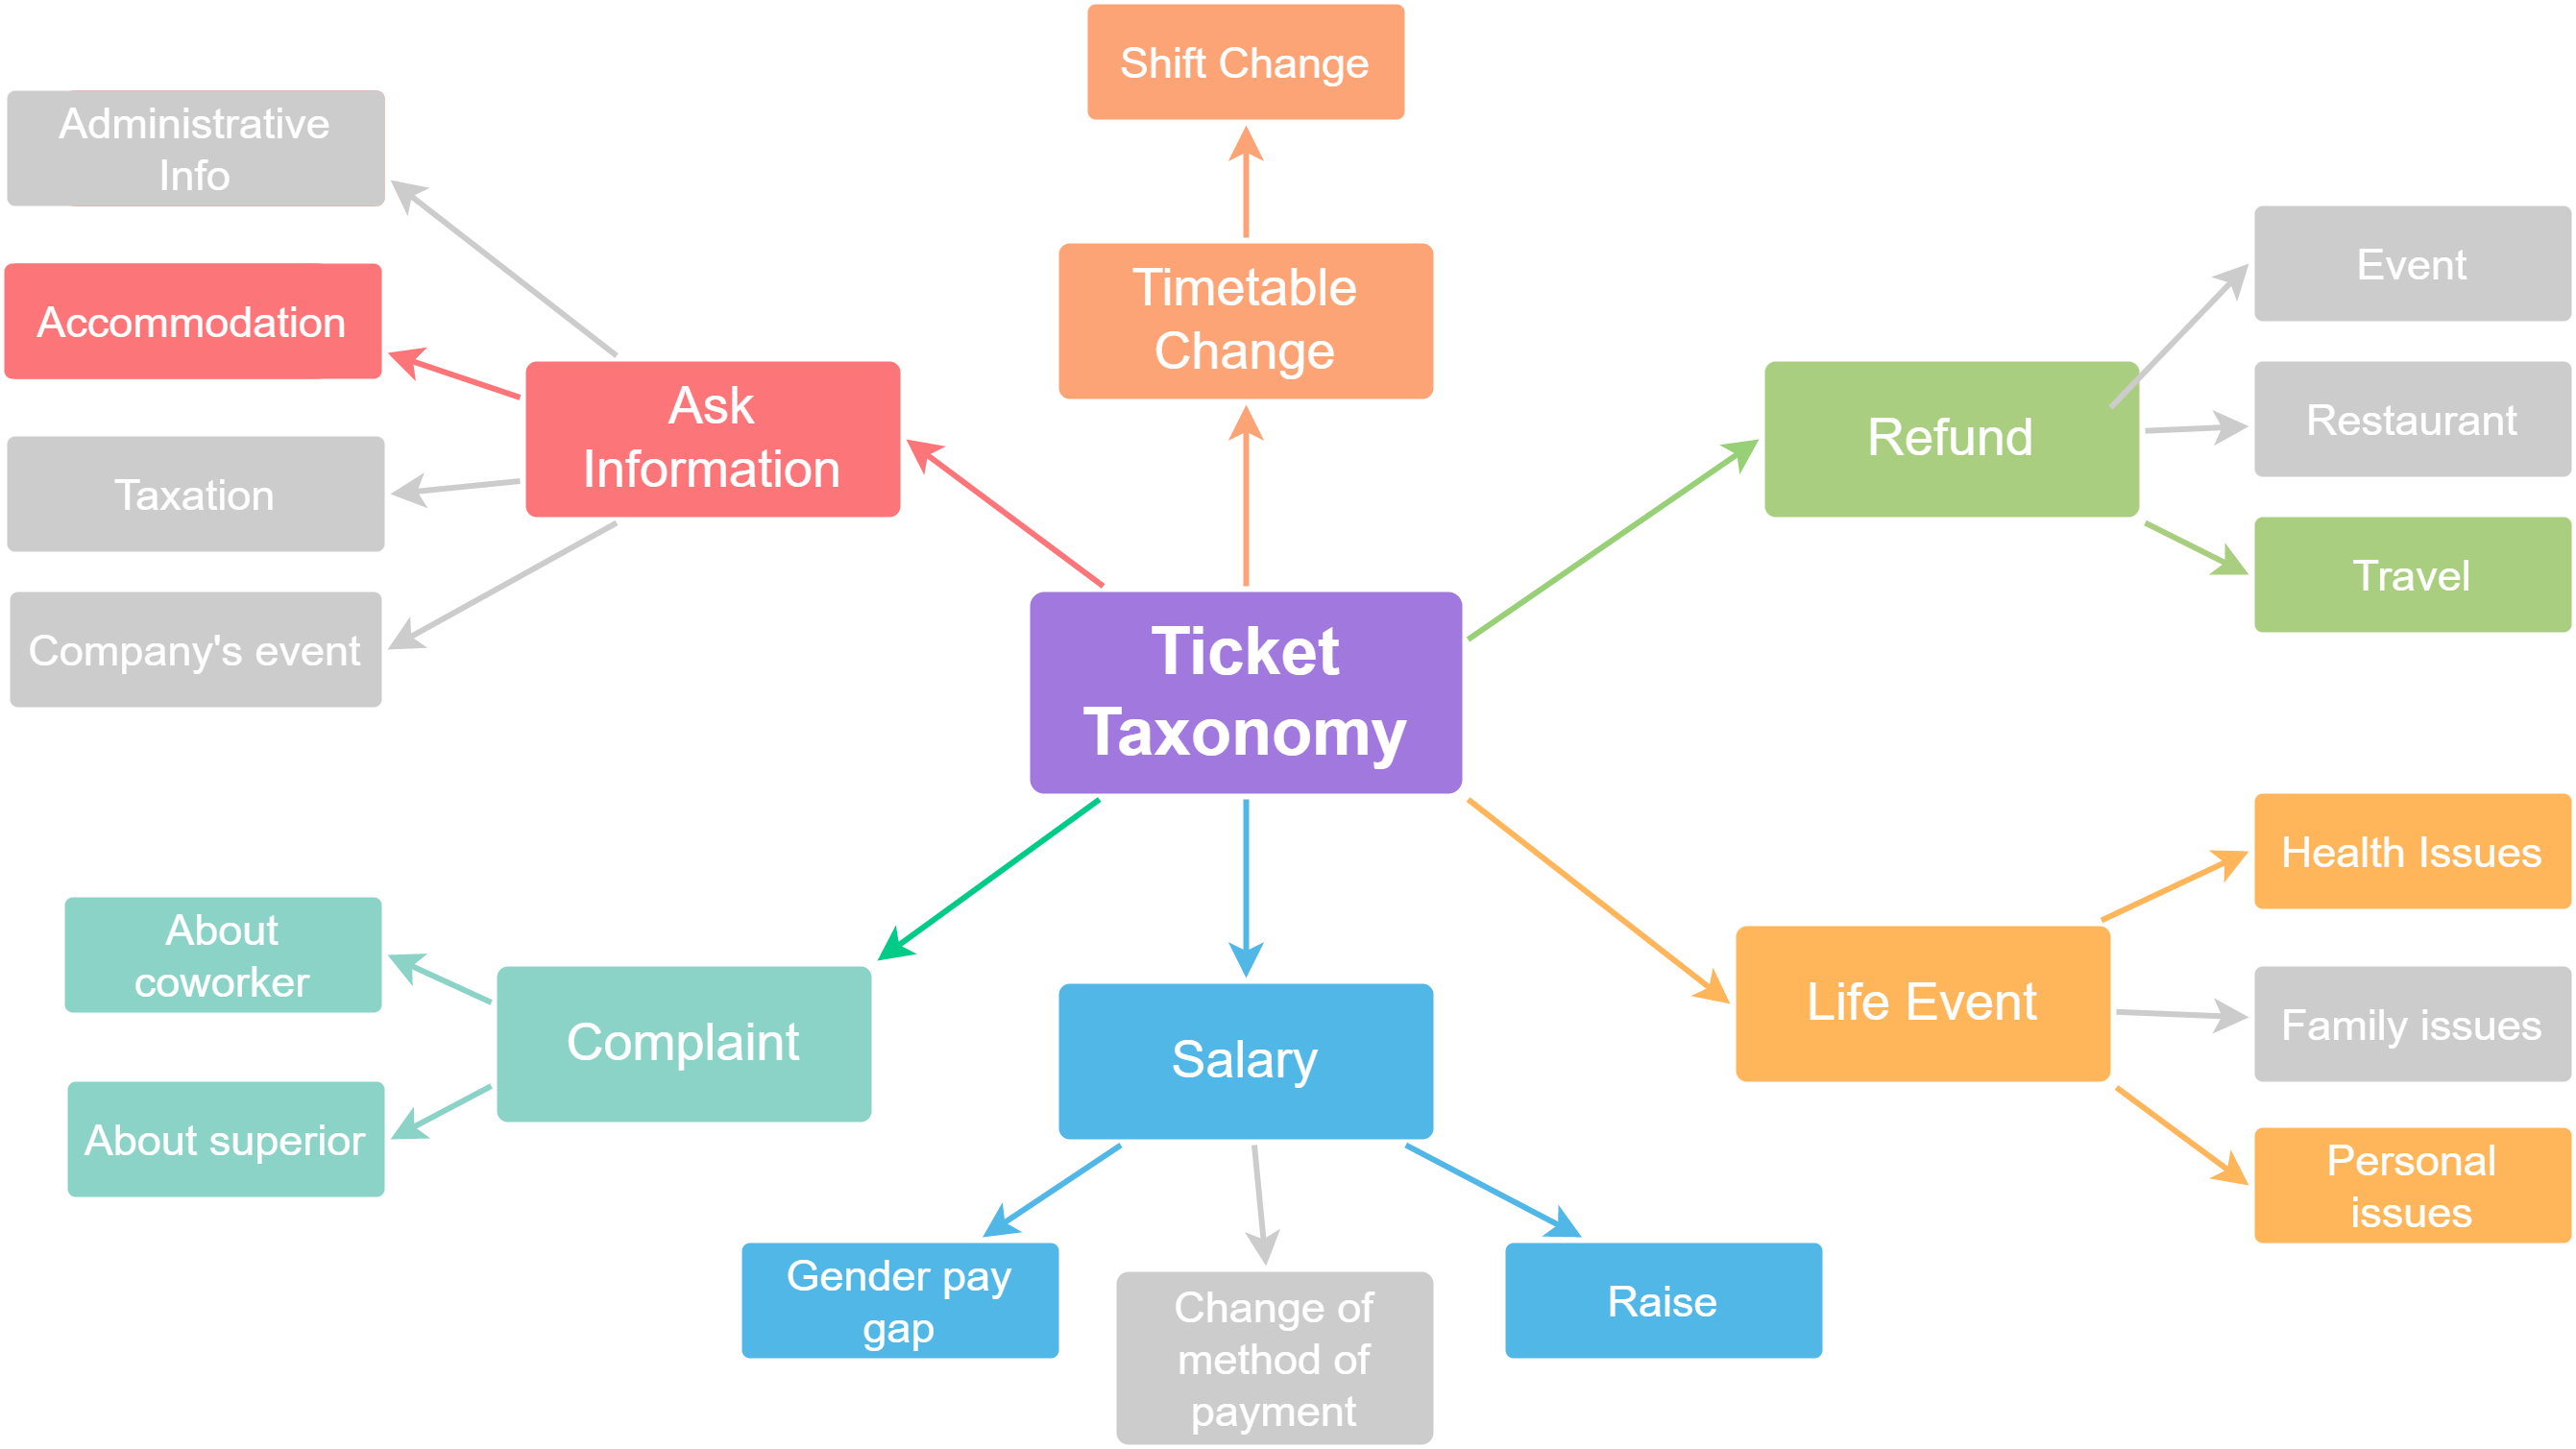
\includegraphics[width=\textwidth]{images/Taxonomy_Tickets_implemented.drawio.png}
    \caption{Final taxonomy, reduced due to unavailability of data}
    \label{fig:final_taxonomy}
\end{figure}    

Usually, HR tickets can belong to various categories, which can range from a request for a shift change to a complaint about a superior. \\
We built a taxonomy of tickets, which is structured into categories and subcategories. Each subcategory has its own variables that are used as inputs for the tickets' generation. The variables are sampled from real-world datasets. \\
For example, to create a request for sick leave, we pass as inputs to our model the reason and the number of days of sick leave requested, which will be acquired from an external dataset. \\
We have a selection of templates and prompts to kick-start the generation process. Every category has its own distinct templates and prompts. The taxonomy (Shown in \autoref{fig:taxonomy} ) has been built following the general structure of the taxonomy of SAP HR tickets, however, the final taxonomy ( Shown in \autoref{fig:final_taxonomy} ) presented here is a subset of the original one due to the unavailability of public data on certain topics ( Ex. \textit{Work benefits}) \\ The final complete taxonomy and the complete list of all variables used for each category/sub-category can be seen in the \autoref{table:categoriesTable}


\begin{table}[h]
    \resizebox{\textwidth}{!}{
    \begin{tabular}{|l|l|l|}
    \hline
        Category            & Sub-category   & variables                                   \\ \hline
        Ask Information     & Accommodation   & location, duration                          \\
        Complaint           & About coworker & complaint, reason                           \\
                            & About superior & complaint, reason                           \\
        Timetable change    & Shift change   & reason\_of\_change, old\_date, new\_date    \\
        Salary              & Salary raise   & old\_salary, new\_salary, increase,work\_title \\
                            & Gender pay gap & wage\_gap                                   \\
        Life Event          & Health issues  & disease, number\_of\_days\_of\_sick\_leave  \\
                            & Personal issues  & issue, number\_of\_days                   \\
        Refund              & Travel         & from, to, date\_travel                     \\
    \hline
    \end{tabular}
    }
\caption{Table of all defined categories and sub-categories with their respective variables}\label{table:categoriesTable}
\end{table}
\section{Datasets}
In order to generate tickets, we decided to use real data as a starting point to make them as much realistic as possible. Another reason to use real data is that it makes the dataset useful for use cases such as anonymization. \\
The dataset that we used are all public and available online. In some cases where no datasets were available, we created them manually from personal experience. \\
The datasets are:
\begin{itemize}
    \item \textit{Absenteeism at work Data Set}: contains records of work absences, with the reason of the absence (almost always a disease) and the number of hours of absence. It is used to create the requests of days off for health reasons
    \item \textit{National Occupational Employment and Wage Estimates United States}: estimates of wages in the US calculated with data collected from employers in all industry sectors in metropolitan and nonmetropolitan areas in every state and the District of Columbia. It is used to create the requests of salary raise.
    \item \textit{List of events of life}: list of major events in life. It is used to create the requests of time off due to personal reasons. 
    \item \textit{Gender pay gap in the UK}: dataset of employers with 250 or more employees, comparing men and women’s average pay across the organizations. It is used to create the requests of explanation for the wage gap amongst genders.
    \item \textit{OpenFlights database}: datasets of airports and flights all over the world. It is used for the requests of refund of travels.
    \item \textit{Geonames all cities with a population over 1000}: datasets of all cities of the world with a population over 1000 people. It is used for the requests of information about accommodation.
\end{itemize}
\subsection{Datasets preprocessing}
The \textit{Absenteeism at work Data Set} is the only dataset that contains data about people that is not already grouped and averaged. This means that there is a record in the dataset for each employee request, which contains the personal information of the employee, the reason for the absence and the time of absence in hours. For privacy reasons, we used a Bayesian Network. \\ 
A Bayesian network is a probabilistic graphical model that measures the conditional dependence structure of a set of random variables based on the Bayes theorem. The features that we have used to build the Bayesian network are the \textit{reason for absence}, the \textit{month of absence} and the \textit{time of absence}.
\\
Using the \textit{Absenteeism at work Data Set} we learn conditional probability distributions from data, to which we add a Laplace noise for differential privacy. Then we can sample new data that follow the original distributions, but that are not equal to the original ones. \\
The absence reasons in the dataset are given as ICD(International Classification of Diseases) codes, to make them more human-readable, we picked for each ICD code the corresponding more frequent diseases. \\
In the \textit{National Occupational Employment and Wage Estimates United States} dataset, we sample employees based on the number of people employed in a certain field. Therefore for example since `Retail Sales Workers` consists of 5.4\% of the total occupations, then the sampled employee will have the 5.4\% of possibility to have as occupation `Retail Sales Worker`. \\
The current salary of the employee is calculated by adding Gaussian noise to the average salary of the employee's occupation, and then the salary raise requested is picked randomly between 5\%-10\%. \\
The ranges of the wage gap, used in the tickets regarding the explanation for the gender wage gap in the company, are sampled randomly from the dataset \textit{Gender pay gap in the UK}, adding a Gaussian noise for privacy reasons. \\
To sample the cities for the requests of accommodation, we randomly sample from all the cities with more than 100,000 inhabitants from the country of residence of the synthetic employee. To calculate the duration of the accommodation we pick a random number of months between 1 and 12. \\
To get data for the category type `refund travel`, we sample randomly one flight from all the flights leaving from the country of the synthetic employee. The data are taken from the \textit{OpenFlights database}. \\
The complaints about coworkers and superiors and the life events that can affect the work life of a person were written by myself, using primarily personal experience and some help from internet blogs.
\subsection{Bayesian Network}\todo{it would be good to cite \link{https://dl.acm.org/doi/abs/10.1145/3134428}}
A Bayesian network is a machine learning method that combines a probabilistic graphical model with Bayesian inference to infer the likelihood of certain events or outcomes. It is used to find relationships between variables and to identify which variables are most influential in predicting a certain outcome or event. \\
The bayesian network is based on the Bayesian theorem:
\begin{equation*}
    p(A|\;B) = \frac{p(B|\;A)p(A)}{p(B)}
\end{equation*}

Formally, the Bayesian network is a directed acyclic graph G = (V,E) with
\begin{itemize}
    \item A feature for each node i belonging to V
    \item A conditional probability distribution for each edge, so the edge from feature $i$ to $j$ represents $p(x_j|\;x_i)$
  \end{itemize}
The base version of a Bayesian network works with discrete variables, however, some implementations consider also continuous variables \cite{chen2017learning} \\
Building a Bayesian network starting from the \textit{Absenteeism at work Data Set} is relatively easy, we calculate the likelihood distribution $p(x_i|\;x_j)\;\forall\:x_i, x_j \in D$, where $D$ is the set of features. As a prior, we used a Dirichlet distribution, mainly because it is the conjugate prior of the categorical distribution. \\
We then added pseudo counts to the observed counts in the data used to calculate $p(x_j|\;x_i)$. This technique is used to diminish the overfitting of data. The values we used for pseudocount is $\gamma=1$. \\
Since we learn the conditional probability distribution from our data, the structure of the network or the conditional probabilities may therefore leak some information on an individual in the dataset. In order to provide strong privacy guarantees and minimize the re-identification risk, we leverage the notion of differential privacy: we perturb the data adding a noise sampled from a Laplace distribution 
\begin{equation*}
    z \sim Laplace \left(0, \frac{2 \cdot n_{features}}{\gamma \cdot \epsilon} \right)
\end{equation*}
where $\epsilon$ is the privacy budget for differential privacy, which controls the anonymization level. \\
Differential privacy is a rigorous mathematical definition of privacy. An algorithm is said to be differentially private if by looking at the output of an algorithm $A$ performed on a dataset $X$, one cannot tell whether any individual's data was included in the original dataset or not. In other words, a differentially private algorithm guarantees that its behavior hardly changes when a single individual joins or leaves the dataset.
The mathematical definition of differential privacy is:
\begin{equation*}
    Pr[A(X) \in Z] \leq e^{\epsilon} \cdot Pr[A(X') \in Z]
\end{equation*}
where $A$ is an algorithm and $X'$ is a neighbour dataset of $X$. A dataset is a neighbor of another dataset if they differ by only one record. \\ 
Once the private Bayesian network is built, we can sample new values for all the nodes in the graph. These generated values will have the same distribution and preserve the consistency and statistical properties of the original dataset up to the noise addition which acts as a de-identification barrier. 

\section{Ticket Generation}
For each HR ticket, we create a synthetic employee. For all tickets' categories, the employee has some common features: \textit{name}, \textit{first name}, \textit{last name}, \textit{nationality}, \textit{country}, \textit{email}, \textit{company}, \textit{company's email} and \textit{ticket date}.\\
All these information are created exploiting the Python library \textit{Faker}. The nationality and the company's country are selected from the extendible list \{ USA, Germany, Italy, Spain, France \}. All other information are created accordingly to the country picked. So for example if the country of birth of the employee is Italy, then the generated name will be Italian. \\
Then, once the employees are generated, the information specific to the ticket category, created starting from the open datasets as mentioned before, are concatenated to the general information of the employees. \\
For each ticket category there are distinct templates. In each template there is an initial part that contains the general information of the employee, such as name, surname, company\dots, then some prompts correlated to the category of the ticket and then the textual prompt. \\
Here's a couple of examples of templates:\\ \\
Request of time off due to health reason:
\begin{adjustwidth}{1cm}{}
From: \$\{email\} \\
To: \$\{company email\} \\
First name: \$\{first name\}\\
Last name: \$\{last name\}\\
Company: \$\{company\}\\
Date: \$\{ticket date\}\\
Ticket category: \$\{category\}\\
Ticket sub-category: \$\{sub category\} \\
Date start absence: \$\{date start absence\} \\
Reason absence: \$\{reason\} \\ 
Subject: Request for sick leave for \$\{number\_of\_days\} \\ 
\\
Dear Sir/Madame, my name is \$\{name\} and I work at \$\{company\}. I am requesting \textless \textit{generate}\textgreater. I hope \textless \textit{generate}\textgreater. \\ \\

\end{adjustwidth}
Request of refund of travel:
\begin{adjustwidth}{1cm}{}
From: \$\{email\} \\
To: \$\{company email\} \\
First name: \$\{first name\}\\
Last name: \$\{last name\}\\
Company: \$\{company\}\\
Date: \$\{ticket date\}\\
Ticket category: \$\{category\}\\
Ticket sub-category: \$\{sub category\} \\
Date Travel: \$\{date\_travel\} \\
From: \$\{airport\_from\}, \$\{from\} \\
Destination: \$\{airport\_to\}, \$\{to\} \\
\\
Hello, my name is \$\{name\}. I am writing this mail to ask a refund for the travel \textless \textit{generate}\textgreater \\ \\

\end{adjustwidth}
        
The variables are replaced with the features of the employee, whereas the \textless \textit{generate}\textgreater \space are replaced with text generated by a generative model. The part generated by the generative model are created in a recursive way. This means that the first \textless generate\textgreater \space is replaced with text generated automatically using as prompt everything that precedes it. Then the second \textless generate\textgreater \space will have as prompt the entire ticket, including the text generated previously by the model. The model is forced to generate some text, if no text is generated in an iteration, the process is repeated until the model gives a non empty output. \\
A general schema of the generation is showed in \autoref{fig:schema_topic_generation}

\begin{figure}[h] 
    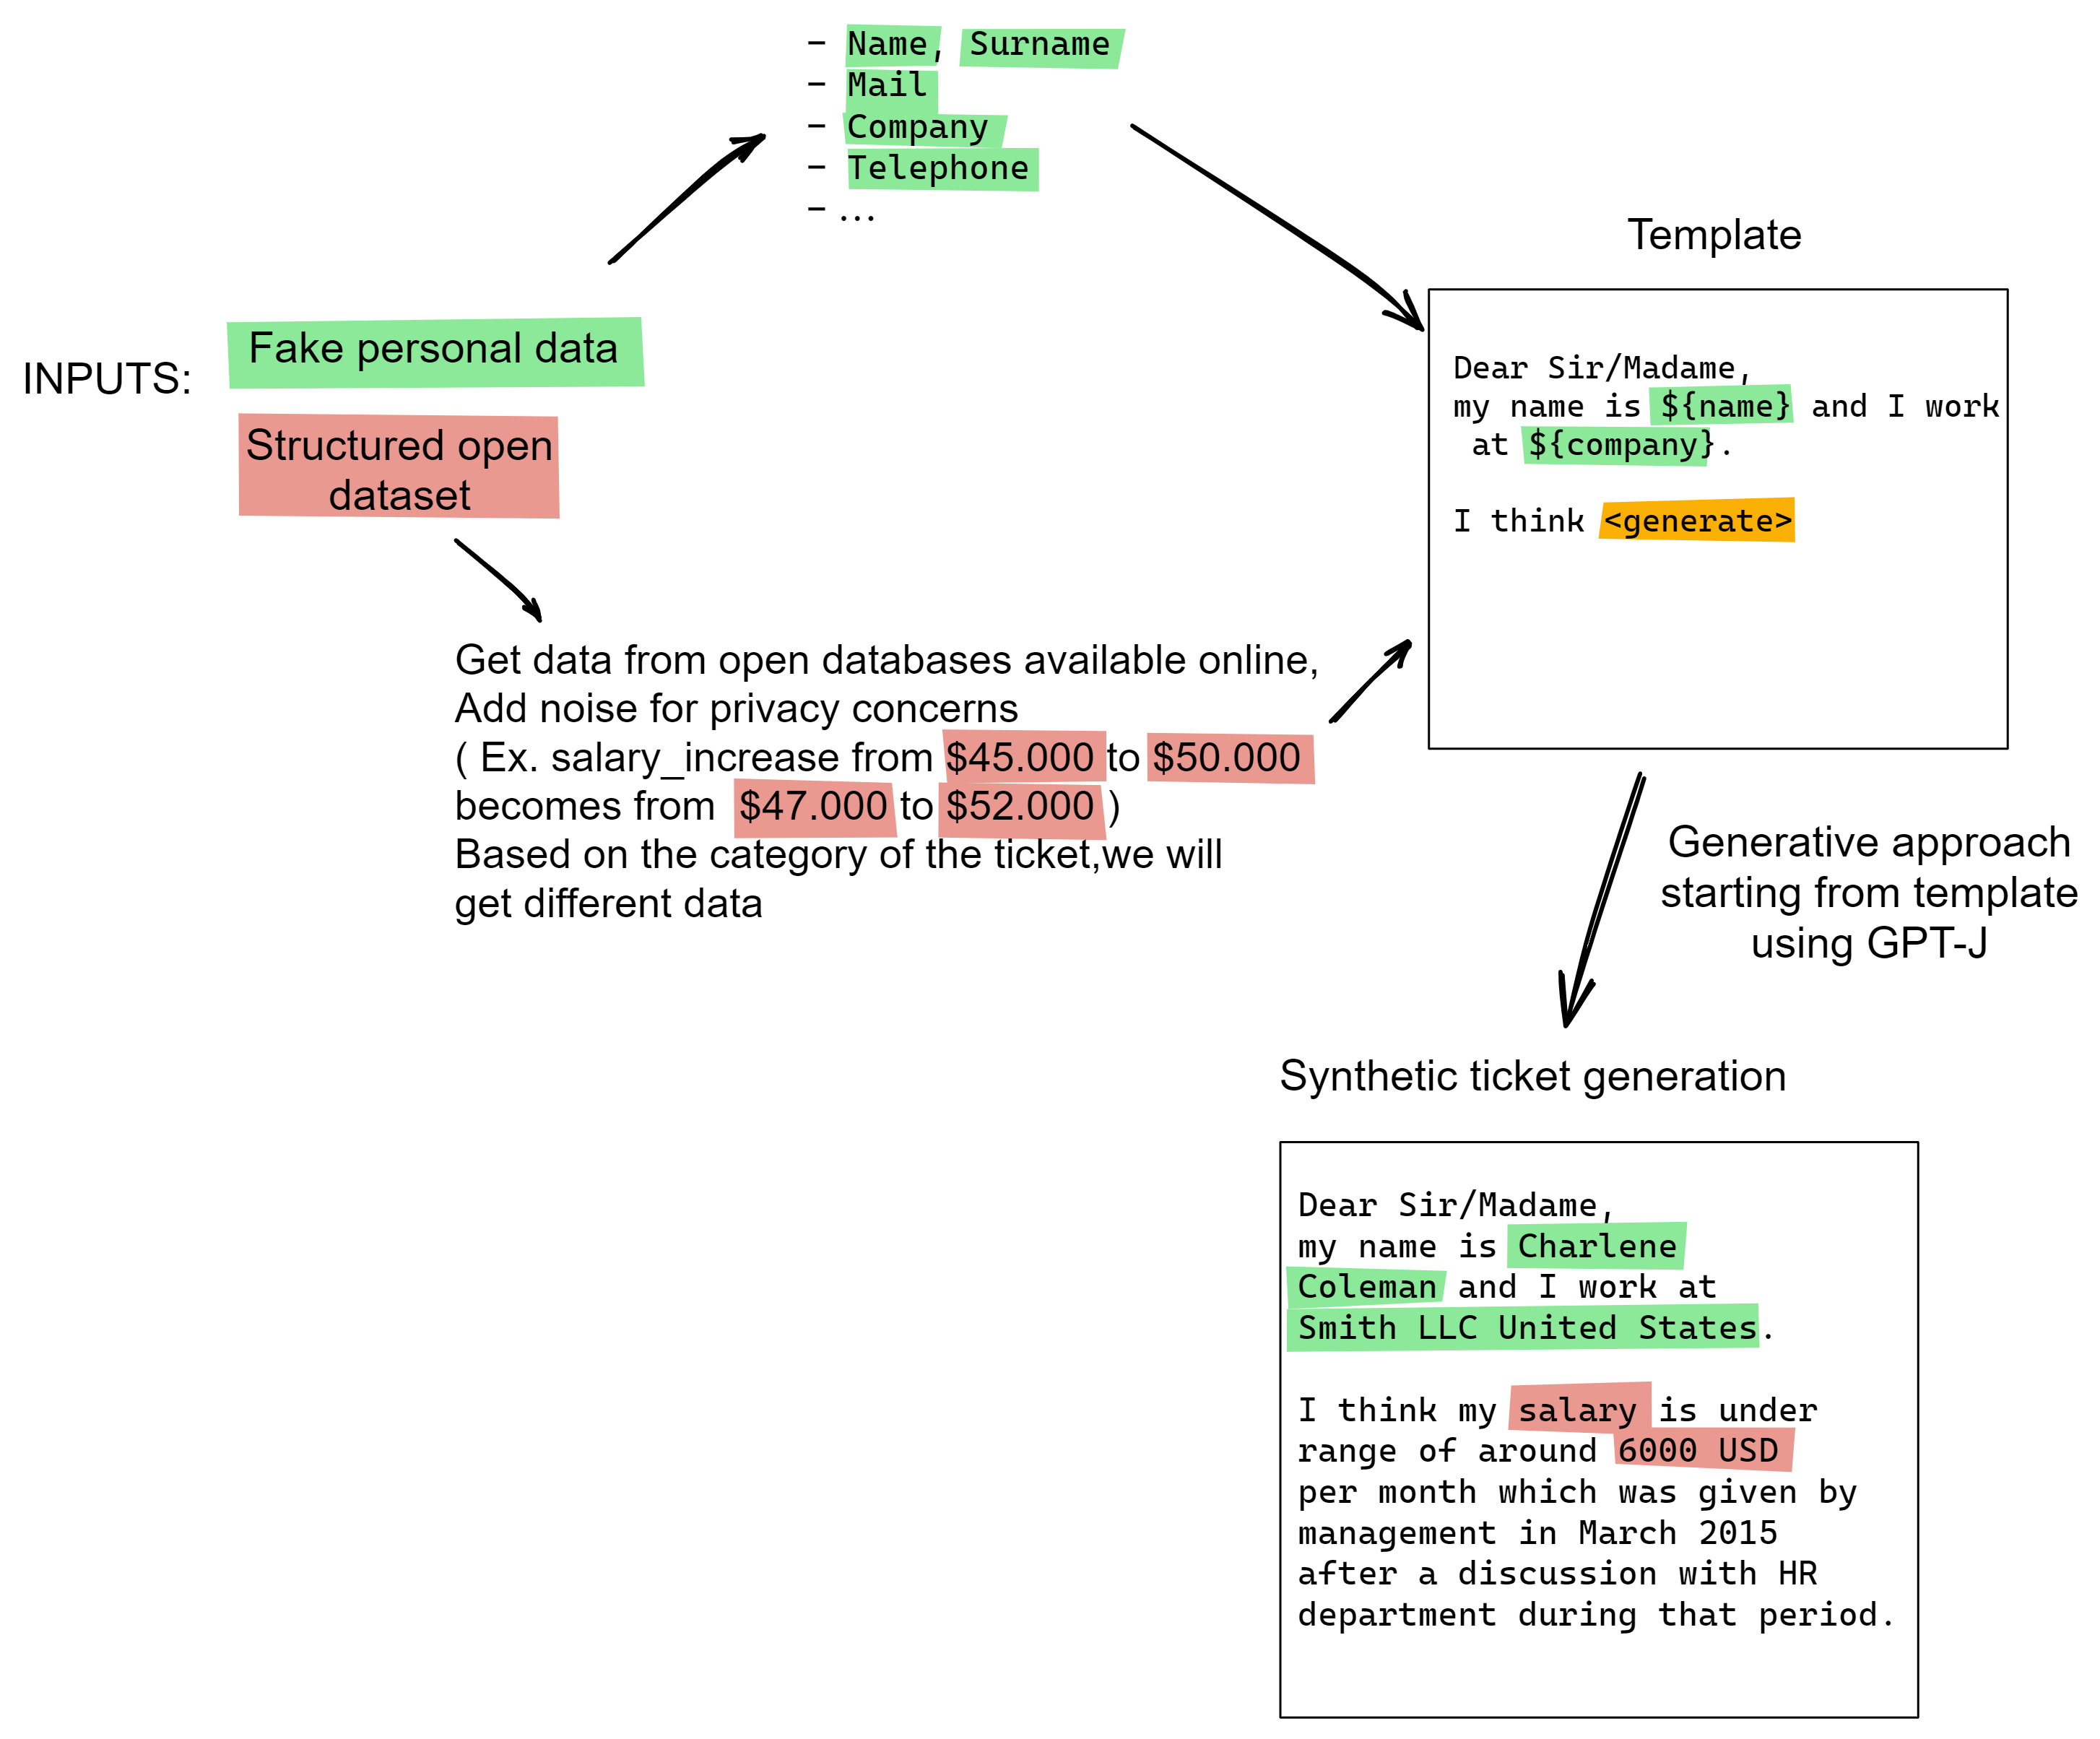
\includegraphics[width=\textwidth]{images/ticket_creation_schema.png}
    \caption{Schema of Ticket Generation}
    \label{fig:schema_topic_generation}
\end{figure}    


\subsection*{Templates}
The model takes in a prompt, or context, and generates text from it. The prompts typically take the form of a few sentences or a paraphrase, and the model generates sentences that fit the context of the prompt. By manipulating the prompt, users can generate text of various tones, topics, and styles. \\
The GPT model is also capable of completing tasks such as question answering, machine translation, and summarization in an unsupervised manner\cite{radford2019language}. By providing a prompt with the task and context, the model can generate accurate results that address the specific context and task. Tasks such as summarization, for instance, require a prompt to provide the model with the information it needs to summarize the text accurately. \\
Changing the prompt of GPT can change the tone, topics, and style of the generated text. Depending on the prompt, GPT can generate text ranging from creative stories to technical summaries. The tone and style of the text can range from humorous to academic, depending on the prompt. As the prompt changes, the model will also adjust to reflect the context of the prompt. \\
This is why we took inspiration from the e-mail format, as HR tickets are created in a working environment where a formal language is used and often they resemble mails in the tone and in the topics. \\
In particular, the Enron Emails dataset is included in the Pile dataset, the dataset which GPT-J is trained on. \\
The emails of the Enron dataset have usually a well-structured prompt, here's an example: 
\begin{adjustwidth}{1cm}{}
    Message-ID: <16593073.1075858228177.JavaMail.evans@thyme>\\
    Date: Wed, 12 Jan 2000 00:29:00 -0800 (PST) \\
    From: carrie.hollomon@enron.com\\
    To: phillip.love@enron.com\\
    Subject: Workhours\\
    Mime-Version: 1.0\\
    Content-Type: text/plain; charset=us-ascii\\
    Content-Transfer-Encoding: 7bit\\\\
    Hello \dots
\end{adjustwidth}
To mimic the format of the emails of the Enron Dataset, we kept the From, To, Date and Subject rows. Instead we removed the Mime-Version, the Content-type and Content-Transfer-Encoding, because after conducting some experiments it was evident that they did not help achieving better results, on the contrary in some cases they were worse. \\
In addition to the standard information, we added explicitly some rows with additional information specific to the category, rather than including them only in the subject or in the initial prompt. \\
\\
In order to generate tickets that were dissimilar and covered a wide range of topics/tokens, we preferred giving to GPT small text prompts and let the model generate most of the text getting the information from the email-like prompt. This approach allowed to improve the diversity of the dataset and, consequently, the usefulness of it. \\
\\
Small text prompt example of a request of shift change:
\begin{adjustwidth}{1cm}{}
    Dear Sir/Madame, my name is \$\{name\}. I wanted to \textless \textit{generate}\textgreater
\end{adjustwidth}

Long text prompt example of a request of shift change:
\begin{adjustwidth}{1cm}{}
    Dear Sir/Madame, my name is \$\{name\} and I work at \$\{company\}. I wanted to ask to change the shift from \$\{old\_date\} to \$\{new\_date\} in order to be able to \textless \textit{generate} \textgreater
\end{adjustwidth}

% TODO: change name of subsection
\subsection*{Architecture analysis}
To understand better how the model was behaving and why it gave certain types of outputs rather than others, we used the python library Ecco, which creates interactive visualization that show at which layers of the architecture the final token has been decided, which input tokens contribute the most for a prediction, \dots \\
In particular, we used two different methods:
\begin{itemize}
    \item Input Saliency: used to show how much did each input token contribute to producing the output token
    \item Neuron Activation Analysis: used to examine underlying patterns in neuron activations using non-negative matrix factorization
\end{itemize}
\subsubsection*{Input Saliency}
To get a better grasp of the most useful information of the prompt, and to understand how we could modify it to achieve better results, we used Gradient * input (Shrikumar et. al). This technique calculates the partial deratives off the output of the model and multiply them with the input itself. Then the inputs with the highest scores are the one that influenced the most the generation of the new tokens
\begin{equation*}
    score = x_i \bigtriangledown f(x_i)
\end{equation*}
where $f$ is the architecture output. \\
The main problem with the Gradient * input method is that only one input is considered. Integrated Gradients solve this issue, computing the average gradient while the input varies along a linear path.
\begin{equation*}
    score = (x_i - x_i')\int_{\alpha = 0}^{1} \bigtriangledown f(x' + \alpha(x - x')) \,d\alpha 
\end{equation*}
Nevertheless, we used the Gradient * input method for computational issues ( The Integrated Gradients took too much RAM of the GPUs ).\\
In the images under we underline some of the considerations we have done while defining the prompts.

\begin{figure*}[h!] 
    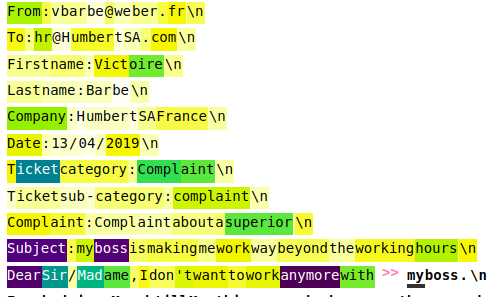
\includegraphics[width=0.6\textwidth]{images/Screenshot from 2022-11-26 17-19-27}
    \caption{Input Saliency: First token}
    \medskip
    \footnotesize
    To create the first token, the model focus on the elements that resembles the content of an email, in particular on the fact the it is indeed a 'Ticket'
    \label{fig:first_token}
\end{figure*}    

\begin{figure*}[h!] 
    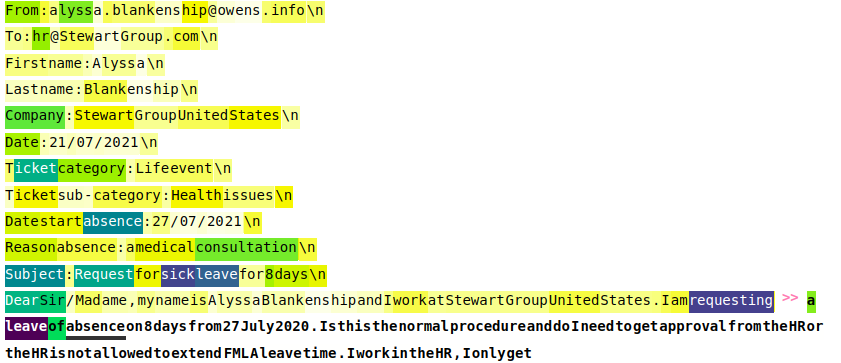
\includegraphics[width=0.8\textwidth]{images/Screenshot from 2022-11-26 18-18-28}
    \caption{Input Saliency: Subject}
    \medskip
    \footnotesize	
    Clearly stating the subject of the ticket helps the model creating tokens that are on the right topic ( In this example 'days of absence')
    \label{fig:topic}
\end{figure*}    

\begin{figure*}[h!] 
    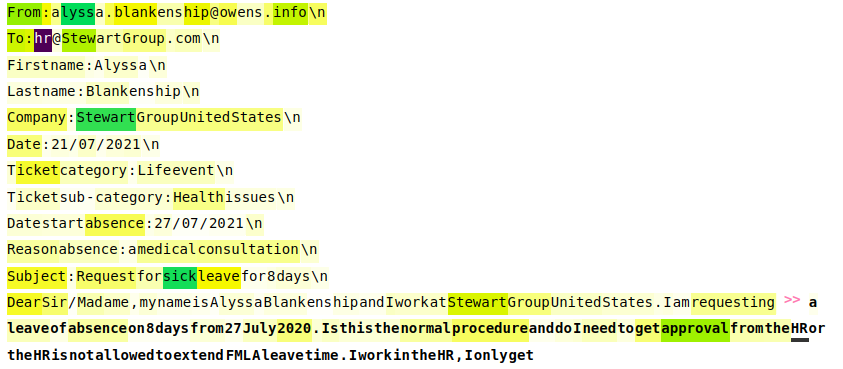
\includegraphics[width=0.85\textwidth]{images/Screenshot from 2022-11-26 18-18-40.png}
    \caption{Input Saliency: HR}
    \medskip
    \footnotesize
    Clearly stating that we are writing to hr can help the model know the context, and consecutively use a certain language, specific words\dots
    \label{fig:hr}
\end{figure*}    


\subsubsection*{Neuron Activation Analysis}
The Feed Forward Neural Network layer is one of the major components inside a transformers block. To better understand how the neurons of different layers were 'activated' and how the neurons contributed towards each generated token, we exploited the Factor Analysis provided by Ecco. \\
Firstly, Ecco calculates the activation scores of each neurons over all layers, and then uses Non-negative Matrix Factorization\ref{fig:nmf} to do dimensionality reduction on the matrix of activations, which will be reduced to a matrix $M{\times}T$, where $M$ is a parameter we decide and $T$ is the number of tokens, starting from a matrix $ ( n \cdot N ){\times}T$, where $n$ is the number of neurons per layer and $N$ is the numbes of layers.
In GPT-J  $n = 16384$ and $N = 28$. \\
Then, for each factor, which are the dimensionality reduced layers, we visualize their activated neurons.
From the example in the \autoref{fig:Neuron_Activation_Analysis}, we can show for each factor what their main contributions are:
\begin{enumerate}
    \item Punctuation
    \item Mail prompt ( From, To, First Name, Last Name, Company\dots)
    \item New lines
    \item Dates
    \item First token, common across various GPT factors
    \item Medical terms ( generally terms related to the tickets' topic )
    \item People's names and contacts
    \item Company's name and contacts
    \item Ticket's subject ( Category, Sub-category and additional info )
    \item Email presentation ( 'Dear Sir/Madame\dots' )
\end{enumerate}

\begin{figure*}[h!] 
    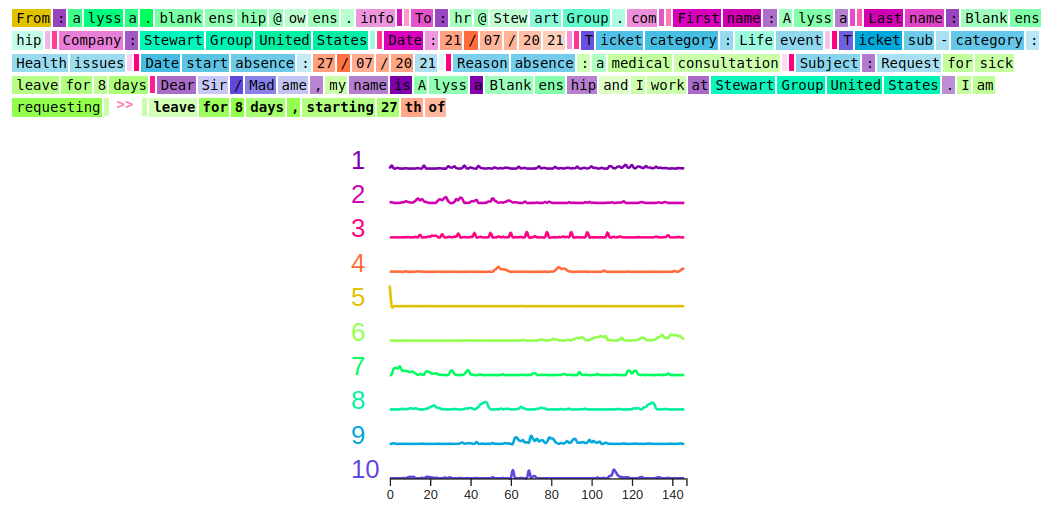
\includegraphics[width=\textwidth]{images/Screenshot from 2022-11-28 15-26-01.png}
    \caption{Neuron Activation Analysis}
    \label{fig:Neuron_Activation_Analysis}
\end{figure*}    


\begin{figure*}[h!] 
    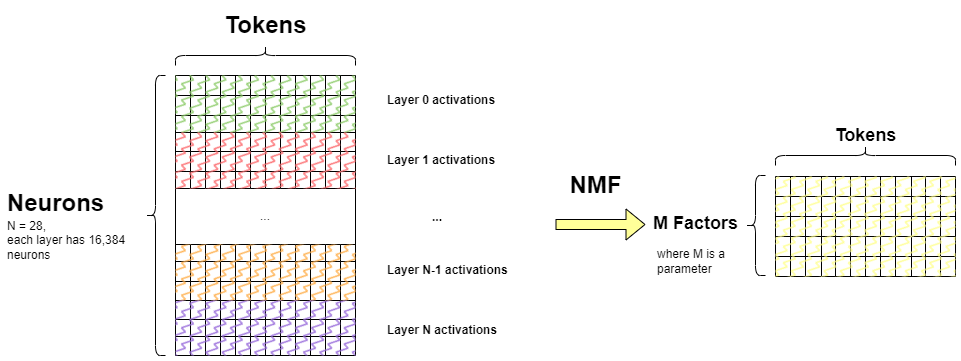
\includegraphics[width=\textwidth]{images/nmf.drawio}
    \caption{Non-negative Matrix Factorization on Activation Matrix}
    \label{fig:nmf}
\end{figure*}    

\section{State of The Art auto-regressive language model}
Autoregressive transformer-based Large Language Models are sequence-to-sequence deep learning models that are pre-trained on a large corpus of data. They are designed to generate new tokens conditioning the model on some input text. The output probability distribution for the next token that the model generates is a probability distribution over all possible tokens in the corpus. \\
Autoregressive transformer-based Large Language Models have shown ability to solve many tasks\cite{gpt3}, varying from more classical ones like translation and question-answering to more peculiar ones, like common sense reasoning and reading comprehension. \\
Mathematically, language models seek to maximize the likelihood of seeing some sentence by considering the product of conditional probabilities up to the point of generation
\begin{equation}
    p(w_T|\;\theta) = \prod_{i=1}^{T}p(w_i|\;w_{1,..,i-1}, \theta)
\end{equation}
Here we list some of the most popular auto-regressive language models:
\begin{itemize}
    \item \textbf{GPT-3}: GPT-3\cite{brown2020language} is an unsupervised AI language model developed by OpenAI. It is the successor to the previous iteration of GPT-2, and when released was the largest language model ever created. GPT-3 first showed that LLMs can be used for few-shot learning across different domains and can achieve state of the art results without building a task-specific model.
    \item \textbf{PaLM}: Pathways Language Model\cite{chowdhery2022palm} is a a 540-billion parameter LM developed by Google. The model was trained through the use of Pathways, a new system that enables highly efficient training of very large neural networks across thousands of TPUs. PaLM few-shot evaluation can outperform or match the finetuned state of the art on a wide array of reasoning tasks.
    \item \textbf{Chinchilla}: Chinchilla\cite{hoffmann2022training} is a LM released by DeepMind. The peculiarity of Chinchilla is that it has 'only' 70B parameters, but outperforms models such as GPT-3 (175B). The authors of the paper demonstrate that for the same computing budget a smaller model trained on more data will perform better.
    \item \textbf{GPT-J}: GPT-J\cite{gptj} is an open-source alternative to OpenAI's GPT-3, the model was released by Eleuther AI, a group of independent researchers and has 6B parameters
    \item \textbf{BLOOM}: BLOOM\cite{scao2022bloom} is an open-source auto-regressive LM released by HuggingFace. BLOOM has a stronger focus on languages, differentiating itself from the majority of other LMs that mainly focus on the English language. In total, BLOOM was trained in 46 different languages
\end{itemize}
Amongst all of these LMs, we picked GPT-J, mainly because it was open-source, free and not too big for our GPU memories\todo{I propose ``more lightweight and thus more convenient in case of productive usage''}. The other main alternative we have tried was GPT-2\cite{radford2019language}, the predecessor of GPT-3, which is now free to use. However, GPT-J's generated text was more coherent and more fluent \\

% TODO: add example of text generated by GPT-J and gpt 2
\todo[inline]{you can also just say that after a comparisative analysis, GPT-L was chosen for the following reasons: }



\section{GPT-J}
\label{sec:gpt_j}

The generative model used to create the tickets is GPT-J, an open source 6 billion parameter, autoregressive text generation model trained on The Pile dataset released by EleutherAI. \\
The Pile dataset\cite{gao2020pile} is an 825 GiB English text corpus composed by 22 diverse subsets, which can be grouped in 5 categories:
\begin{itemize}
    \item Academic ( \textit{ArXiv}, \textit{PubMed Central}, ... )
    \item Internet ( \textit{Wikipedia}, \textit{StackExchange}, ... )
    \item Prose ( \textit{Bibliotik}, ... )
    \item Dialogue ( \textit{Subtitles}, ... )
    \item Misc ( \textit{Github}, ... )
\end{itemize}
\subsection{Parameters}
\label{sec:parameters}
The parameters used for the generation of the next token are:
\begin{itemize}
    \item \textit{min\_length}: minimum number of words created by a round of gpt generation
    \item \textit{max\_length}: maximum number of words created by a round of gpt generation.  
    \item \textit{top\_k}: the k most likely next words are filtered and the probability mass is redistributed among only these k words. It helps the model not to go off-topic.
    \item \textit{top\_p}: the next words are sampled from the smallest possible set of words whose cumulative probability exceeds the probability p. Compared to \textit{top\_k}, in this case the size of the set of possible next token is not fixed. In practice, usually \textit{top\_k} and \textit{top\_p} are used together.
    \item \textit{temperature}: the value $T$ used to module the logits distribution. The higher the value of $T$, the higher the entropy of the logits distribution will be. In other words, tokens with an high probability will be less probable and tokens with a low probability will be more probable.
    \begin{equation*}
        p_i = \frac{exp(x_i/T)}{\sum_j exp(x_j/T)}   
    \end{equation*}
    \item \textit{repetition\_penalty}: the parameter $\theta$ for repetition penalty. 1.0 means no penalty \\
    Given a list of generated tokens $G$, 
     \begin{equation*}
        p_i = \frac{exp\left(\frac{x_i}{T \cdot I(i \in G)}\right)}{\sum_j exp\left(\frac{x_j}{T \cdot I(j \in G)}\right)}
    \end{equation*}
    \begin{center}
    $I(c) = \theta$ if $c$ is True else 1
    \end{center}    
    So the logits distribution of the token changes based on if the token has already been generated before.

    \item \textit{length\_penalty}: \textit{length\_penalty} $>$ 0 promotes longer sequences, while \linebreak 
    \textit{length\_penalty} $<$ 0 encourages shorter sequences.

    \item \textit{no\_repeat\_ngram\_size}: If set to an integer $>$ 0, all ngrams of that size can only occur once \\
    Ex: \textit{no\_repeat\_ngram\_size} = 2 \\
    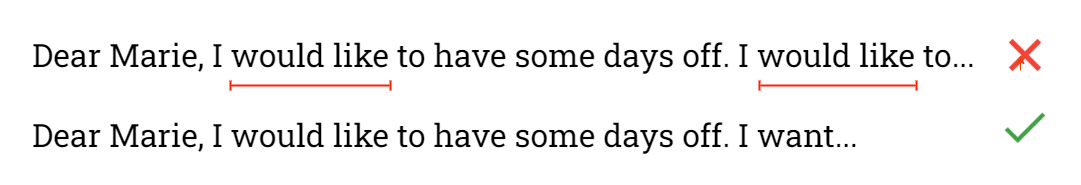
\includegraphics[width=0.94\textwidth]{images/no_ngram_thesis.drawio.png}

    \item \textit{num\_beams}: Number of beams for beam search. They beams are the number of 'paths' that are considered when choosing the next token. Even if a token is not the one with the highest probability, it can be chosen as the next token if the complete sentence is considered as more probable than the alternatives. \\
    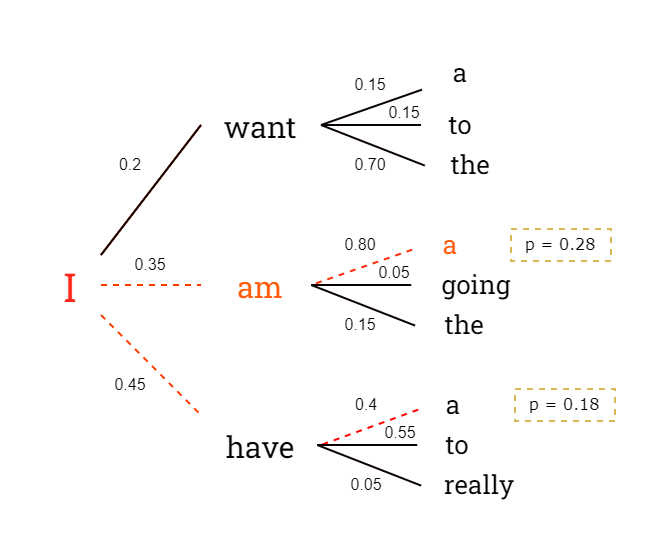
\includegraphics[width=0.6\textwidth]{images/num_beams.drawio.png}

    \item \textit{do\_sample}: If set to `False` greedy decoding is used ( the most probable token is always chosen). Otherwise, sampling is used ( the next token is chosen sampling from the distribution of possible next tokens )
    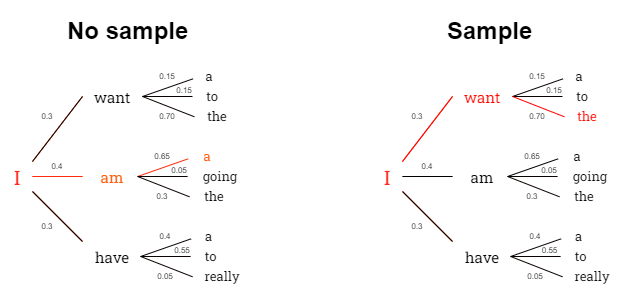
\includegraphics[width=0.90\textwidth]{images/do_sample.drawio.png}

    \item \textit{bad\_words}: List of words that are not allowed to be generated by the model.
    \item \textit{force\_words}: List of words that must be generated in the generation.
    
\end{itemize}
The default values assigned to the parameters used are shown in \autoref{table:parametersGPTJTable}, however the application is set up in order to being able to apply different parameters at each run.

\begin{table}[h] 
\centering
\begin{tabular}{|l|l|}
\hline
Parameter          & Value \\ \hline
min length         & 0    \\ 
max length         & 50    \\ 
top k              & 50    \\
top p              & 0.85  \\
repetition penalty & 1.2   \\
temperature        & 1     \\
length penalty     & 1     \\
no repeat ngram size     & 0     \\
num beams &  1 \\
do sample & True \\
bad words & [\space] \\
force words & [\space] \\ \hline
\end{tabular}
\caption{Parameters of GPT-J model}\label{table:parametersGPTJTable}
\end{table}
\subsection{Architecture}
The GPT architecture is based on the original Transformers paper. The original architecture introduced two types of transformers blocks: the encoder block and the decoder block. \\
The encoder block converts an input sequence of tokens into a sequence of embedding vectors, whereas the decoder takes the output of the encoder and generate iteratively an output sequence of tokens. \\
GPT is pre-trained by predicting the next word based on the previous ones. \\
GPT is decoder-only, which means that is assembled only by a stack of decoder blocks. Each decoder block is composed by:
\begin{itemize}
    \item \textbf{Normalization Layers}: a normalization layer \cite{ba2016layer} normalize all inputs of a neural network across their features. It has been shown that Layer normalization enables smoother gradients, faster training, and better generalization accuracy \cite{xu2019understanding}

    $x$: data sample \\
    $d$: dimension of data sample \\
    $y$: output of LayerNorm \\
    $\epsilon$: small number added for stability

    \begin{equation*}
        u = \frac{1}{d}\sum_{i=1}^{d}x_i 
    \end{equation*}
    \begin{equation*}
        \sigma^2 = \frac{1}{d}\sum_{i=1}^{d}(x_ - ui)^2
    \end{equation*}
    \begin{equation*}
        \hat{x_i} = \frac{x_i - u}{\sqrt{\sigma^2 + \epsilon}}
    \end{equation*}
    \begin{equation*}
        y = \gamma\hat{x_i} + \beta
    \end{equation*}

    where $\gamma$ and $\beta$ are parameters that the model learns.
    \item \textbf{Masked Self-Attention Layer}: attention is a mechanism that allows neural networks to assign a different amount of weight to each token in a sequence and process each token as a weighted average of all other tokens. \\
    In practice three matrixes are calculated:
    \begin{itemize}
        \item $Q$ (Query): the representation of the current token
        \item $K$ (Key): the representation of all the other tokens, which are matched with the current token
        \item $V$ (Value): the representation of all the words, used for the weighted-average
    \end{itemize}
    The $Q$, $K$ and $V$ matrixes are initialized as:
    \begin{itemize}
        \item $Q$ = $W_qX + b_q$ 
        \item $K$ = $W_kX + b_k$ 
        \item $V$ = $W_vX + b_v$
    \end{itemize}
    where $X$ is the input matrix and the other matrixes are randomly initialized and learned by the model.
    Finally, the attention score is calculated with
    \begin{equation*}
        Attention(Q,K,V) = softmax \left(\frac{QK^T}{\sqrt{d}}\right)V
    \end{equation*}
    where $d$ is a normalization factor equivalent to the embeddings' dimension \\
    The masked self-attention is a modified version of self-attention where all the tokens that appear after the current one are set to $0$, in order not to let the model being influenced by any information regarding the tokens at the next positions. This is fundemental when training generative models such as GPT, whose scope is to predict the successive tokens.
    \begin{equation*}
        Attention(Q,K,V) = softmax\left(\frac{QK^T + Mask}{\sqrt{d}}\right)V
    \end{equation*}

    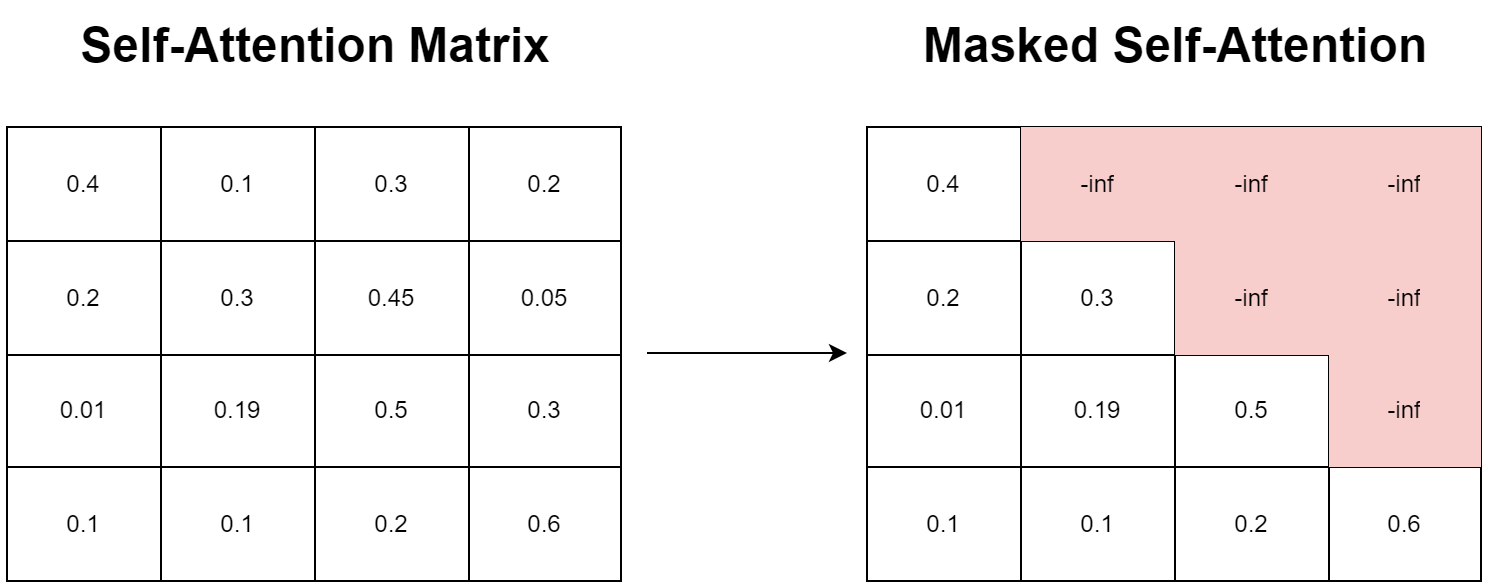
\includegraphics[width=0.90\textwidth]{images/masked_self_attention.drawio.png}

    \item \textbf{Feed Forward Neural Network Layer}: Used to add non-linearity to the transformer block
\end{itemize}

\begin{figure}[h] 
    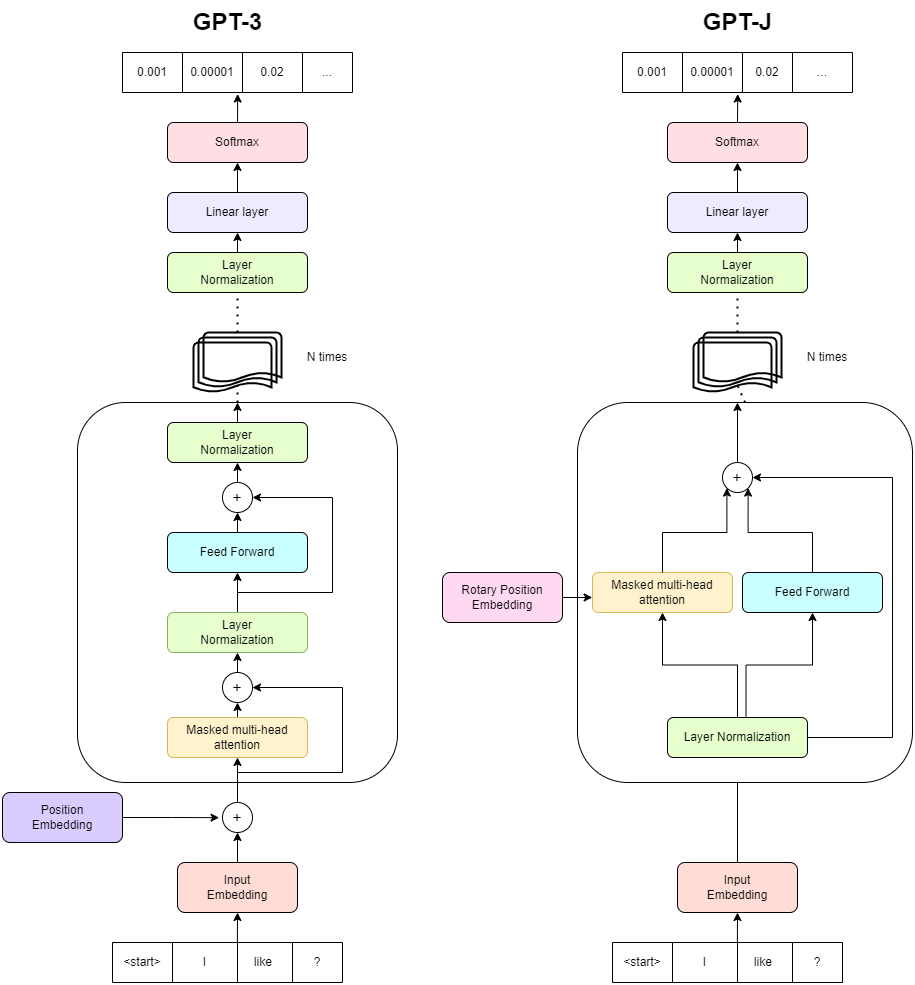
\includegraphics[width=\textwidth]{images/gptJ_vs_gpt_architecture.drawio.png}
    \caption{GPT-3 and GPT-J architectures compared}
    \label{fig:gpt-architectures}
\end{figure}    

\begin{figure}[h] 
    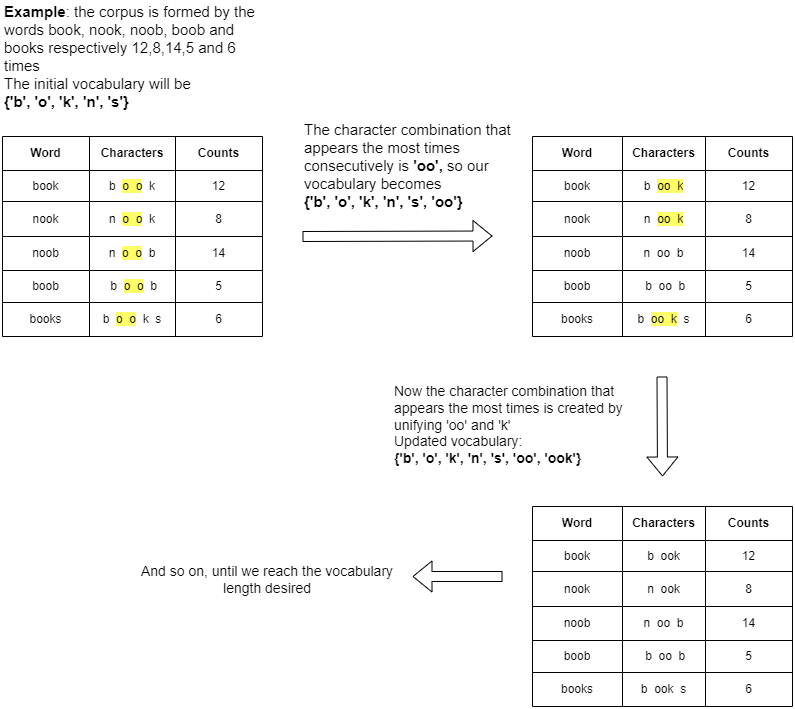
\includegraphics[width=\textwidth]{images/byte_pair.drawio.png}
    \caption{Byte-Pair Encoding Tokenization Example}
    \label{fig:Byte_Pair_Encoding}
\end{figure}    


GPT models use a Byte-Pair Encoding tokenization. The Byte-Pair Encoding algorithm starts by building a vocabulary with all the single characters of the corpus we are training on. Then, at each step of the algorithm, the two tokens which appear consecutevily the most in the words of the corpus are unified and create a new token. This process continue until the desired vocabulary lenght is satisfied. An example taken from the site \cite{byte-pair-encoding} is shown in the \autoref{fig:Byte_Pair_Encoding}


Compared to GPT-3, GPT-J\cite{gptj} has two minor architectural differences  ( shown in \autoref{fig:gpt-architectures}):
\begin{itemize}
    \item Rotary Embedding
    \item The attention layer and the feedforward layer in parallel for decreased communication
\end{itemize}

\subsubsection{Rotary Position Embedding}
Position embeddings are used to infer the notion of position to the model, which does not have any sense of position for each token. In other words, using the attention mechanism each token "match" with the other tokens in the same manner, not considering where if the other token is located right after the current one or if it is at the end of the sentence. Position embeddings are used to add to the model this sense of position. \\ Rotary position embedding has been introduced by Su et al.\cite{su2021roformer}, it is a novel method that unifies absolute and relative approaches to position embeddings. \\
The typical approach, which is also used by GPT-3, is to use a sinusoidal embedding, which is defined as
\begin{equation*}
    \begin{cases}
        p_{1,2t} = sin(k/10000^{2t/d}) \\
        p_{1,2t+1} = cos(k/10000^{2t/d}) 
    \end{cases}
\end{equation*}
where $p_{1,2t}$ is the $2^{th}$ element of the d-dimensional vector $p_i$
RoPE instead proposes to incorporate the relative position information by multiplying the context representation with the sinusoidal functions instead of directly adding them. \\
If we define 
\begin{equation*}
    \begin{split}
        q_m = f_q(x_m, m) \\
        k_n = f_k(x_n, n) 
    \end{split}    
\end{equation*}

where $f_q$ and $f_k$ are functions that incorporate the $m^{th}$ and $n^{th}$ positions respectively to the vector embeddings $x_m$ and $x_n$ to produce the query and key vectors, we can require the inner product of the query $q_m$ and $k_n$ to be formulated by a function $g$ that depends only on the word embeddings $x_m$, $x_n$ and their relative position $m - n$
\begin{equation*}
    \langle f_q(x_m, m) \: , \: f_k(x_n, n) \rangle = g(x_m,x_n,m-n)
\end{equation*}
In the simplest case $d=2$, $f_{\{q,k\}}$ are defined as
\begin{equation*}
    f_{(\{q,k\}, \{m,n\})} = (W_{\{q,k\}}x_{\{m,n\}})e^{i\{m,n\}\theta}
\end{equation*}
and therefore we obtain
\begin{equation*}
    g(x_m, x_n, m - n) = Re[(W_qx_m)(W_kx_n)^Te^{i(m-n)\theta}]
\end{equation*}
which preserves the relative positional information of the word embeddings. This equation is used when calculating the self-attention, which will become
\begin{equation*}
    Attention(Q,K,V) = softmax\left(\frac{g(x_m, x_n, m - n)}{\sqrt{d}}\right)V
\end{equation*}
This equation can be generalized for $d > 2$, as shown in the original paper. \\
In the end, incorporating the RoTE is pretty straightforward, you just have to rotate the word embedding by a multiple of its position index. \\
According to the researchers that published GPT-J\cite{rope-eleutherai}, using RoTE leads to a faster convergence of training and validation losses and a lower overall validation loss.

\noindent
\begin{minipage}{\linewidth}
    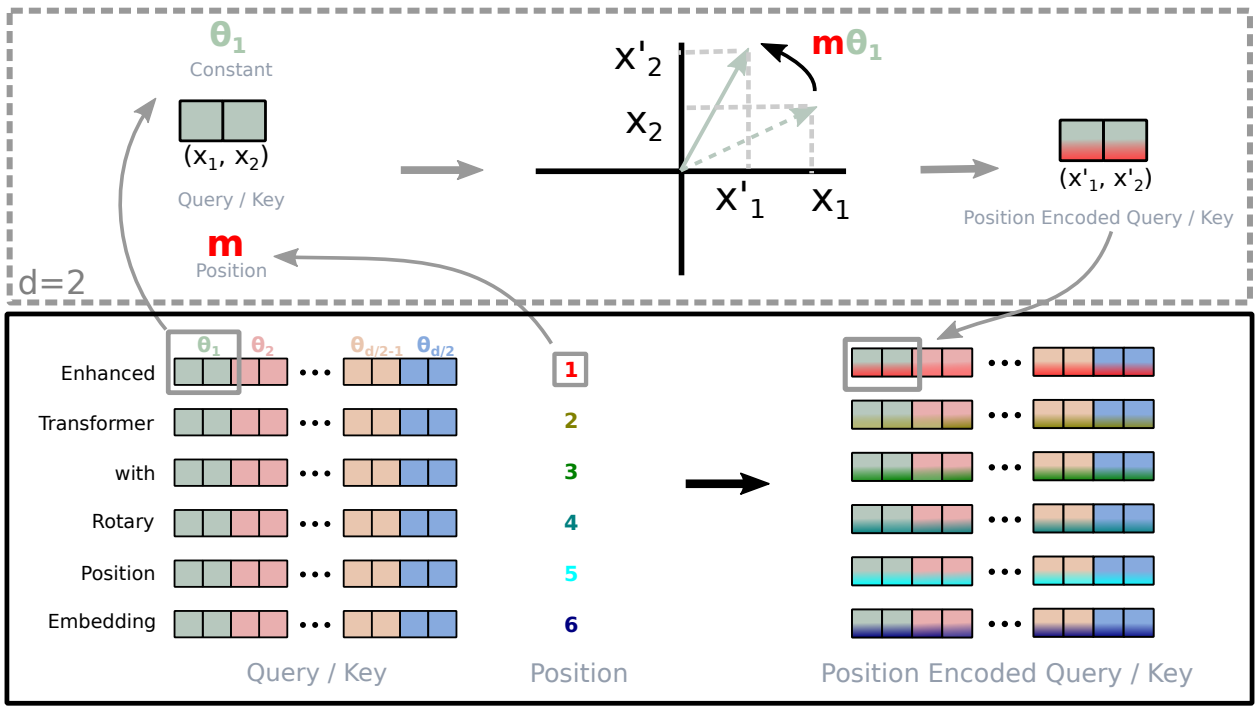
\includegraphics[width=\linewidth]{images/rotary_embedding_from_paper.PNG}
    \captionof{figure}{Implementation of RoPE, Image taken from original paper\cite{su2021roformer}}
\end{minipage}%
\section{Architecture analysis}
To understand better how the model was behaving and why it gave certain types of outputs rather than others, we used the python library Ecco\cite{alammar-2021-ecco}, which creates interactive visualizations that show at which layer of the architecture the final token has been decided, which input tokens contribute the most for a prediction, and many other insights on the model. \\
In particular, we used two different methods:
\begin{itemize}
    \item \textbf{Input Saliency}: used to show how much did each input token contribute to producing the output token
    \item \textbf{Neuron Activation Analysis}: used to examine underlying patterns in neuron activations using non-negative matrix factorization
\end{itemize}
\subsubsection*{Input Saliency}
To get a better grasp of the most useful information of the prompt, and to understand how we could modify it to achieve better results, we used the Gradient * input\cite{shrikumar2017learning} method. This technique calculates the partial derivatives of the output of the model and multiplies them with the input itself. Then the inputs with the highest scores are considered the ones that influenced the most the generation of the new tokens
\begin{equation*}
    score = x_i \bigtriangledown f(x_i)
\end{equation*}
where $f$ is the architecture output. \\
The main problem with the Gradient * input method is that only one input is considered. Integrated Gradients\cite{sundararajan2017axiomatic} solve this issue, computing the average gradient while the input varies along a linear path.
\begin{equation*}
    score = (x_i - x_i')\int_{\alpha = 0}^{1} \bigtriangledown f(x' + \alpha(x - x')) \,d\alpha 
\end{equation*}
Nevertheless, we used the Gradient * input method for computational issues ( The Integrated Gradients took too much RAM of the GPUs ).\\
In the images under, we underline some of the considerations we have done while defining the prompts.

\begin{figure*}[h!] 
    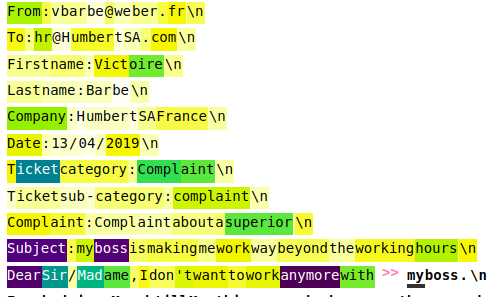
\includegraphics[width=0.6\textwidth]{images/Screenshot from 2022-11-26 17-19-27}
    \caption{Input Saliency: First token}
    \medskip
    \footnotesize
    To create the first token, the model focus on the elements that resemble the content of an email, in particular on the fact that it is indeed a 'Ticket'
    \label{fig:first_token}
\end{figure*}    

\begin{figure*}[h!] 
    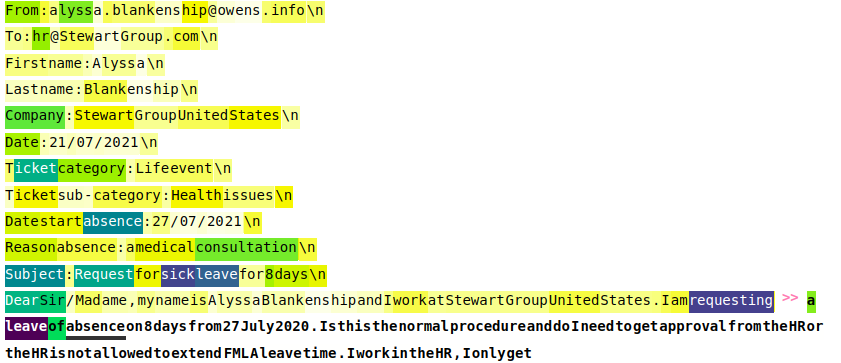
\includegraphics[width=0.8\textwidth]{images/Screenshot from 2022-11-26 18-18-28}
    \caption{Input Saliency: Subject}
    \medskip
    \footnotesize	
    Clearly stating the subject of the ticket helps the model create tokens that are on the right topic ( In this example 'days of absence')
    \label{fig:topic}
\end{figure*}    

\begin{figure*}[h!] 
    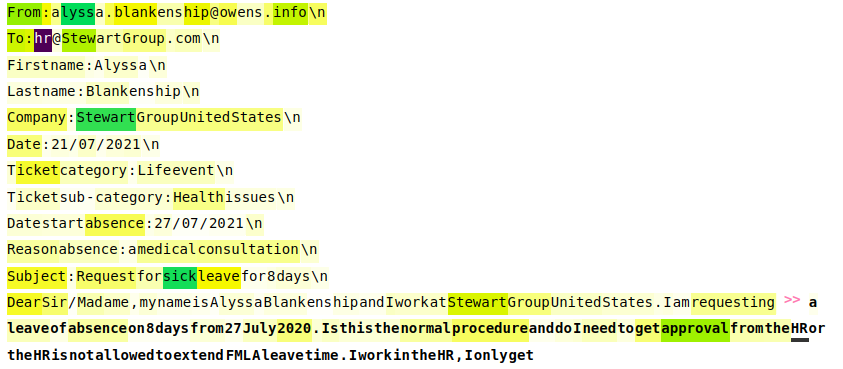
\includegraphics[width=0.85\textwidth]{images/Screenshot from 2022-11-26 18-18-40.png}
    \caption{Input Saliency: HR}
    \medskip
    \footnotesize
    Clearly stating that we are writing to hr can help the model know the context, and consecutively use a certain language, specific words\dots
    \label{fig:hr}
\end{figure*}    


\subsubsection*{Neuron Activation Analysis}
The Feed Forward Neural Network layer is one of the major components inside a transformer's block. To better understand how the neurons of different layers were 'activated' and how the neurons contributed towards each generated token, we exploited the Factor Analysis provided by Ecco. \\
Firstly, Ecco calculates the activation scores of each neuron over all layers, and then uses Non-negative Matrix Factorization (\autoref{fig:nmf}) to do dimensionality reduction on the matrix of activations, which will be reduced to a matrix $M{\times}T$, where $M$ is a parameter we decide and $T$ is the number of tokens, starting from a matrix $ ( n \cdot N ){\times}T$, where $n$ is the number of neurons per layer and $N$ is the number of layers. In GPT-J  $n = 16384$ and $N = 28$. \\
\begin{figure*}[h] 
    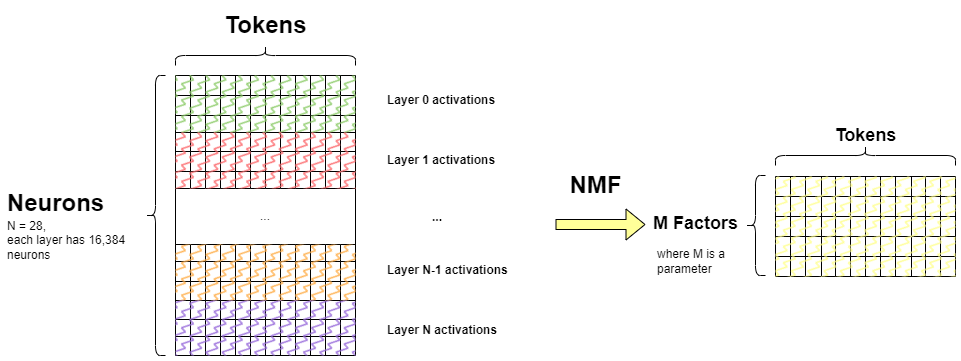
\includegraphics[width=\textwidth]{images/nmf.drawio}
    \caption{Non-negative Matrix Factorization on Activation Matrix}
    \label{fig:nmf}
\end{figure*}
Then, for each factor, which are the dimensionality-reduced layers, we visualize their activated neurons.
From the example in the \autoref{fig:Neuron_Activation_Analysis}, we can show for each factor what their main contributions are:
\begin{enumerate}
    \item Punctuation
    \item Mail prompt ( From, To, First Name, Last Name, Company\dots)
    \item New lines
    \item Dates
    \item First token, common across various GPT factors
    \item Medical terms ( usually terms related to the tickets' topic )
    \item People's names and contacts
    \item Company's name and contacts
    \item Ticket's subject ( Category, Sub-category and additional info )
    \item Email presentation ( 'Dear Sir/Madame\dots' )
\end{enumerate}

\begin{figure*}[h] 
    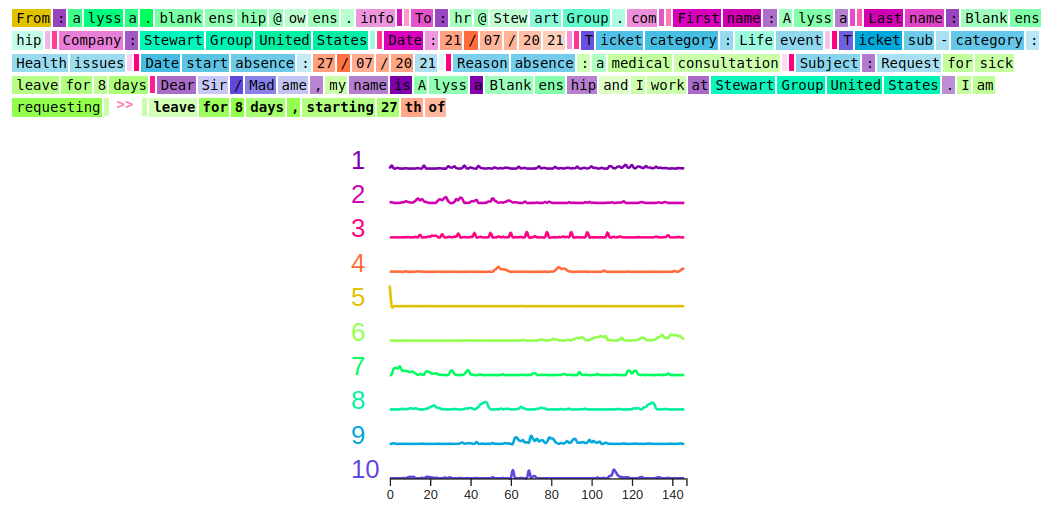
\includegraphics[width=\textwidth]{images/Screenshot from 2022-11-28 15-26-01.png}
    \caption{Neuron Activation Analysis}
    \label{fig:Neuron_Activation_Analysis}
\end{figure*}    



\section{Survey}
In order to understand whether the tickets were similar to real tickets, we conducted a survey internal to the company. We were not able to get real data from the company's HR due to the sensitive nature of the data.\todo[inline]{In order to avoid any ethical implications, we decided to conduct our assessment without involving any real personal data or situations.} \\
We asked all our\todo{to some} colleagues to \todo[inline]{act as the automatic text generator, filling} fill out a form in an Excel file, where the users were given twenty random prompts, similar to the ones that are given to the GPT model. \\
After giving a brief explanation of the project and what we were trying to achieve, we recommended the users not to use their personal information while writing the fake tickets, but to use the same style of text and the same vocabulary they would use in a real situation. \\
For each ticket, there were several information attached that appeared over all the tickets, which were: name of the person, category of the ticket, sub category of the ticket and some information that were specific to the ticket's category, for example for the category-sub\_category 'Salary - Salary Raise' the additional information given was the new requested salary. \\
We asked the users not to use necessarly all the information that were present in the prompts, but only the ones that felt natural to use, and to slightly change them if it made sense to them ( Ex: Sick leave from Oct 20 2022 can become 'from this Thursday, the 20') \\
Each user was given twenty different prompts sampled randomly from a set of 800 total prompts, belonging to the same categories-sub\_categories of our taxonomy. The prompts contained only the contextual information of the ticket and no ticket's text, so, unlike the prompts used for the GPT models, there were no initial text such as 'Dear Sir/Madame, I would like to \dots' \\
The respondent were also asked to tick the information that they used, and these information were supposed to be used as testing in the NER use case. However, many people either did not tick any information or they ticked only partially what they used, therefore in the end we did not make use of these data. \\\\

\begin{figure}[!h] 
    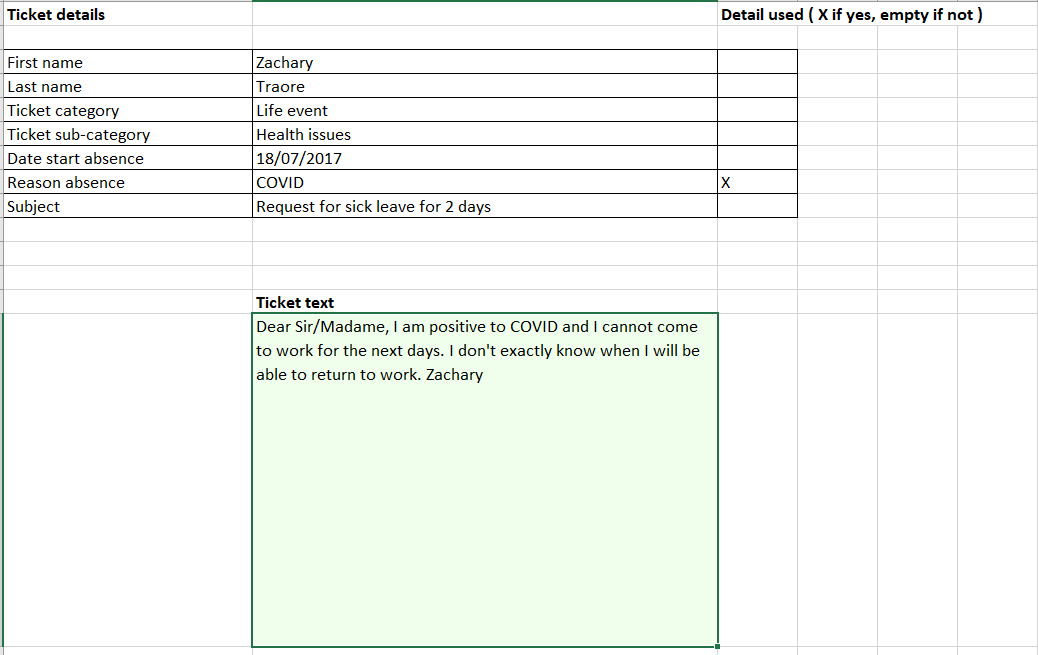
\includegraphics[width=\textwidth]{images/excel_schema_v2.PNG}
    \caption{Example of survey}
    \label{fig:survey}
\end{figure}    



\section{Results}
In this section we analyze the created dataset, comparing it to the tickets we collected from the survey. \\
The final dataset of HR tickets automatically generated is composed by exactly 16,000 tickets, 2000 for each category. On the other hand, we collected 259 test tickets from 29 different respondents. \\
To evaluate the generation of the tickets, we have used a handful of traditional unsupervised text evaluation techniques. We were not able to exploit more complex classical metrics, such as BLEU and ROUGE, not having real data as references for each prompt.
The reported metrics are:
\begin{itemize}
    \item avg ttr unigram: average TTR(type token ratio) for the unigrams of the tickets\\ 
    \begin{equation*}
        TTR = \frac{number\_of\_unique\_unigrams}{total\_number\_of\_unigrams}
    \end{equation*}
    \item avg ttr bigram: average TTR(type token ratio) for the bigram of the tickets\\ 
    \begin{equation*}
        TTR = \frac{number\_of\_unique\_bigrams}{total\_number\_of\_bigrams}
    \end{equation*}
    \item avg ratios of nouns: average ratio of nouns in the tickets\\
    \begin{equation*}
        noun\_ratio = \frac{counter\_noun\_words}{counter\_all\_words}
    \end{equation*}
    \item avg ratios of verbs: average ratio of verbs in the tickets\\
    \begin{equation*}
        verb\_ratio = \frac{counter\_verb\_words}{counter\_all\_words}
    \end{equation*}
    \item avg\_word\_frequency: average frequency of words, using as frequency estimates a dump of the English version of Wikipedia, considering only words appearing at least 10 times\\
    \begin{equation*}
        word\_freq= 
        \begin{cases}
            log_{e}(word\_freq\_wiki),& \text{if } word\_freq\_wiki\geq 10\\
            skip,                   & \text{otherwise}
        \end{cases}
    \end{equation*}
\end{itemize}
First, we reported the type-token-rations given that high-quality writing has been associated with the presence of more diverse words and phrases\cite{pitler2008revisiting}. We computed them for each ticket and then we averaged the results. \\
Second, since lower frequency words indicate a more advanced output\cite{crossley2011development}, we compute the average word frequency of the generated words.\\
Then, we calculate nouns and verb ratios over sentence length, as indicators of syntactic complexity, and therefore richer text\cite{mcnamara2010linguistic}. To single out nouns and verbs, we use the pre-trained Spacy POS model. \\\\
We report in \autoref{table:initial_results} the results we obtained initially. The metrics have been calculated not only on the tickets generated by the model and the tickets of the surveys, but also on some baseline datasets (\textit{Amazon reviews}, \textit{Reddit comments} and \textit{NIPS papers}). The datasets have been chosen to be as diversified as possible in terms of text longevity, type of language and terms used. \\ %TODO: maybe add for each dataset a brief description
The main takeaways from the metrics are:
\begin{itemize}
    \item The model tends to write more unique words and not to repeat itself, since the average TTR of both unigrams and bigrams are higher in the tickets of the survey
    \item The model tends to use more nouns than a real person
    \item The model tends the same number of verbs as a real person
    \item The average number of words ( word count ) varies a lot from category to category, both in generated and survey tickets
\end{itemize}
We know that these analyses are not completely reliable due to the low number of real data compared to the size of our dataset. However they are a good indication of how to improve the generation. \\
For this reason, we changed the parameters of the ticket creation and recreated the dataset from scratch, in order to be more akin to the survey tickets. \\
The final results are shown in \autoref{table:final_results}. \\
Some of the surveys' metrics change a bit compared to the first table, this is due to some late respondents to the survey, which skewed a little bit the final test metrics.

\begin{table}[h]
    \resizebox{\textwidth}{!}{
    \setlength\extrarowheight{16pt}
    \begin{tabular}{|l|l|l|l|l|l|l|}
    \hline
    Dataset                                                                           & \shortstack{avg ttr\\unigram} & \shortstack{avg ttr\\bigram} & \shortstack{avg ratios\\of nouns} & \shortstack{avg ratios\\of verbs} & \shortstack{avg word\\frequency} & \shortstack{avg word\\count} \\ \hline
    Amazon reviews                                                                    & 0.81                          & 0.98                         & 0.16                              & 0.10                              & 13.86, $\sigma$=0.47               & 73.73, $\sigma$=71.75    \\ \hline
    Reddit comments                                                                   & 0.91                          & 0.99                         & 0.15                              & 0.11                              & 13.33, $\sigma$=1.53               & 37.70, $\sigma$=84.96    \\ \hline
    NIPS papers                                                                       & 0.26                          & 0.72                         & 0.18                              & 0.06                              & 13.50, $\sigma$=0.25               & 5798.40, $\sigma$=737.17 \\ \hline
    Tickets survey & 0.87                                                             & 0.99                          & 0.17                         & 0.11                              & 13.84                             & 42.73, $\sigma$=28.83                  \\ \hline
    Tickets generated by GPT                                                          & 0.93                          & 1.00                         & 0.14                              & 0.10                              & 13.84, $\sigma$=0.35               & 57.87, $\sigma$=19.13    \\ \hline
    \shortstack[l]{Survey\\Salary\_Salary raise}                                      & 0.85                          & 0.99                         & 0.20                              & 0.10                              & 13.85, $\sigma$=0.56              & \textcolor{red}{55.65}, $\sigma$=35.67    \\ \hline
    \shortstack[l]{GPT\\Salary\_Salary raise}                                         & 0.90                          & 1.00                         & 0.15                              & 0.10                              & 13.72, $\sigma$=0.33              & \textcolor{red}{70.73}, $\sigma$=16.36    \\ \hline
    \shortstack[l]{Survey\\Complaint\_Complaint}                                      & 0.83                          & 0.98                         & 0.15                              & 0.13                              & 13.66, $\sigma$=0.91              & 63.64, $\sigma$=46.67    \\ \hline
    \shortstack[l]{GPT\\Complaint\_Complaint}                                         & 0.91                          & 0.99                         & 0.14                              & 0.12                              & 13.94, $\sigma$=0.32              & 72.81, $\sigma$=21.62    \\ \hline
    \shortstack[l]{Survey\\Life event\_Personal issues}                               & 0.89                          & 0.99                         & 0.17                              & 0.12                              & 13.99, $\sigma$=0.56              & \textcolor{red}{33.54}, $\sigma$=19.85    \\ \hline
    \shortstack[l]{GPT\\Life event\_Personal issues}                                  & 0.92                          & 1.00                         & 0.13                              & 0.12                              & 14.08, $\sigma$=0.25              & \textcolor{red}{63.88}, $\sigma$=15.62    \\ \hline
    \shortstack[l]{Survey\\Refund\_Refund travel}                                     & 0.90                          & 0.99                         & 0.17                              & 0.11                              & 13.56, $\sigma$=0.56              & 34.76, $\sigma$=17.02    \\ \hline
    \shortstack[l]{GPT\\Refund\_Refund travel}                                        & 0.96                          & 1.00                         & 0.16                              & 0.08                              & 13.72, $\sigma$=0.38              & 38.91, $\sigma$=10.83    \\ \hline
    \shortstack[l]{Survey\\Timetable change\_Shift change}                            & 0.83                          & 0.99                         & 0.16                              & 0.10                              & 14.16, $\sigma$=0.66              & 38.15, $\sigma$=15.30    \\ \hline
    \shortstack[l]{GPT\\Timetable change\_Shift change}                               & 0.93                          & 1.00                         & 0.13                              & 0.10                              & 13.79, $\sigma$=0.37              & 47.95, $\sigma$=9.72     \\ \hline
    \shortstack[l]{Survey\\Ask information\_Accommodation}                            & 0.88                          & 0.99                         & 0.17                              & 0.11                              & 13.80, $\sigma$=0.50              & 39.93, $\sigma$=23.89    \\ \hline
    \shortstack[l]{GPT\\Ask information\_Accommodation}                               & 0.95                          & 1.00                         & 0.14                              & 0.10                              & 13.68, $\sigma$=0.36              & 47.10, $\sigma$=10.59    \\ \hline
    \shortstack[l]{Survey\\Life event\_Health issues}                                 & 0.90                          & 0.99                         & 0.17                              & 0.13                              & 13.88, $\sigma$=0.44              & \textcolor{red}{31.92}, $\sigma$=14.70    \\ \hline
    \shortstack[l]{GPT\\Life event\_Health issues}                                    & 0.91                          & 1.00                         & 0.14                              & 0.10                              & 13.84, $\sigma$=0.33              & \textcolor{red}{59.07}, $\sigma$=16.06    \\ \hline
    \shortstack[l]{Survey\\Salary\_Gender pay gap}                                    & 0.85                          & 0.97                         & 0.21                              & 0.11                              & 13.87, $\sigma$=0.43              & 53.94, $\sigma$=32.71    \\ \hline
    \shortstack[l]{GPT\\Salary\_Gender pay gap}                                       & 0.93                          & 0.99                         & 0.15                              & 0.11                              & 13.96, $\sigma$=0.28              & 62.52, $\sigma$=18.67    \\ \hline
    \end{tabular}}
    \caption{Initial Results}\label{table:initial_results}
\end{table}



\begin{table}[h]
    \resizebox{\textwidth}{!}{
    \setlength\extrarowheight{16pt}
    \begin{tabular}{|l|l|l|l|l|l|l|}
    \hline
    Dataset                                                                           & \shortstack{avg ttr\\unigram} & \shortstack{avg ttr\\bigram} & \shortstack{avg ratios\\of nouns} & \shortstack{avg ratios\\of verbs} & \shortstack{avg word\\frequency} & \shortstack{avg word\\count} \\ \hline
    Amazon reviews                                                                    & 0.81                          & 0.98                         & 0.16                              & 0.10                              & 13.86, $\sigma$=0.47               & 73.73, $\sigma$=71.75          \\ \hline
    Reddit comments                                                                   & 0.91                          & 0.99                         & 0.15                              & 0.11                              & 13.33, $\sigma$=1.53               & 37.70, $\sigma$=84.96          \\ \hline
    Tickets survey                                                                    & 0.86                          & 0.99                         & 0.17                              & 0.11                              & 13.89, $\sigma$=0.59               & 44.43, $\sigma$=27.46          \\ \hline
    Tickets generated by GPT                                                          & 0.94                          & 1.00                         & 0.14                              & 0.10                              & 13.86, $\sigma$=0.39               & 49.22, $\sigma$=15.49          \\ \hline
    \shortstack[l]{Survey\\Salary\_Salary raise}                                      & 0.84                          & 0.99                         & 0.21                              & 0.10                              & 13.89, $\sigma$=0.52               & 55.10, $\sigma$=32.44          \\ \hline
    \shortstack[l]{GPT\\Salary\_Salary raise}                                         & 0.90                          & 1.00                         & 0.15                              & 0.10                              & 13.73, $\sigma$=0.35               & 62.87, $\sigma$=14.12          \\ \hline
    \shortstack[l]{Survey\\Complaint\_Complaint}                                      & 0.82                          & 0.98                         & 0.15                              & 0.13                              & 13.74, $\sigma$=0.84               & 62.74, $\sigma$=42.83          \\ \hline
    \shortstack[l]{GPT\\Complaint\_Complaint}                                         & 0.92                          & 0.99                         & 0.14                              & 0.11                              & 13.94, $\sigma$=0.33               & 59.46, $\sigma$=18.39          \\ \hline
    \shortstack[l]{Survey\\Life event\_Personal issues}                               & 0.88                          & 0.99                         & 0.17                              & 0.12                              & 14.03, $\sigma$=0.55               & 38.15, $\sigma$=20.86          \\ \hline
    \shortstack[l]{GPT\\Life event\_Personal issues}                                  & 0.94                          & 1.00                         & 0.14                              & 0.11                              & 14.19, $\sigma$=0.30               & 45.49, $\sigma$=16.94          \\ \hline
    \shortstack[l]{Survey\\Refund\_Refund travel}                                     & 0.88                          & 0.99                         & 0.17                              & 0.11                              & 13.61, $\sigma$=0.53               & 37.50, $\sigma$=17.36          \\ \hline
    \shortstack[l]{GPT\\Refund\_Refund travel}                                        & 0.96                          & 1.00                         & 0.16                              & 0.08                              & 13.72, $\sigma$=0.38               & 39.52, $\sigma$=10.46          \\ \hline
    \shortstack[l]{Survey\\Timetable change\_Shift change}                            & 0.83                          & 0.99                         & 0.16                              & 0.10                              & 14.17, $\sigma$=0.62               & 38.73, $\sigma$=14.71          \\ \hline
    \shortstack[l]{GPT\\Timetable change\_Shift change}                               & 0.93                          & 1.00                         & 0.12                              & 0.10                              & 13.74, $\sigma$=0.40               & 42.80, $\sigma$=7.55           \\ \hline
    \shortstack[l]{Survey\\Ask information\_Accommodation}                            & 0.87                          & 0.99                         & 0.16                              & 0.11                              & 13.90, $\sigma$=0.50               & 41.86, $\sigma$=23.79          \\ \hline
    \shortstack[l]{GPT\\Ask information\_Accommodation}                               & 0.95                          & 1.00                         & 0.14                              & 0.10                              & 13.65, $\sigma$=0.38               & 46.79, $\sigma$=10.99          \\ \hline
    \shortstack[l]{Survey\\Life event\_Health issues}                                 & 0.87                          & 0.99                         & 0.17                              & 0.13                              & 13.94, $\sigma$=0.42               & 37.91, $\sigma$=21.80          \\ \hline
    \shortstack[l]{GPT\\Life event\_Health issues}                                    & 0.94                          & 1.00                         & 0.16                              & 0.09                              & 13.95, $\sigma$=0.37               & 43.36, $\sigma$=11.26          \\ \hline
    \shortstack[l]{Survey\\Salary\_Gender pay gap}                                    & 0.85                          & 0.97                         & 0.22                              & 0.11                              & 13.87, $\sigma$=0.41               & 53.14, $\sigma$=31.13          \\ \hline
    \shortstack[l]{GPT\\Salary\_Gender pay gap}                                       & 0.94                          & 1.00                         & 0.14                              & 0.11                              & 13.99, $\sigma$=0.29               & 53.49, $\sigma$=13.51          \\ \hline
    \end{tabular}}
    \caption{Final Results}\label{table:final_results}
\end{table}

% TODO: add self-bleu 

\subsection*{Topic analysis}
Topic modeling is a type of statistical modeling technique used to discover the hidden topics and patterns in a corpus of text. It is a type of unsupervised machine learning method that automatically discovers topics from a collection of documents by analyzing words and phrases in each document. Topics are usually represented by word clusters or distributions that are related to each other. Topic modeling can be used to generate meaningful summaries about large collections of documents. \\
We used topic modeling to visualize in a summarized form the major topics of our dataset and to verify that the topics created correspond to the ones in the taxonomy.\todo[inline]{one could ask how the topic analysis on the manually-produced dataset relates to the generated one, what are similarities/differences etc. The reason is clearly stated but the question may arise, if you have the data, it might be worth including some words on this aspect.} \\
The model of topic modeling we chose is BERTopic\cite{grootendorst2022bertopic}. BERTopic generates document embedding with pre-trained transformer-based language models, clusters these embeddings, and finally, generates topic representations with the class-based TF-IDF\todo[inline]{Term Frequency-Inverse Document Frequency (TF-IDF)} procedure
\begin{algorithm}
    \caption*{BERTopic}
    \begin{algorithmic}[1]
      \State Documents are embedded to create representations in vector space using Sentence-BERT
      \State The embeddings generated are reduced in dimensionality using UMAP
      \State The reduced embeddings are clustering used HDBSCAN. HDBSCAN is a variation of the hierarchical clustering algorithm DBSCAN that models clusters using a soft-clustering approach, allowing noise to be modeled as outliers
      \State The most relevant terms for each topic are found using a class-based version of TF-IDF. All documents in a cluster are treated as a single document by simply concatenating them, so we measure how much information a term provides to a class instead of a document.
      \State If the user requests a number of topics smaller than the number of topics generated, the least common topics are iteratively merged with their most similar topic, until the number of topics requested is satisfied.
    \end{algorithmic}
\end{algorithm}

The formula of the class-based TF-IDF is:
\begin{equation*}
    W_{t,c} = tf_{t,c} \cdot \log(1 + \frac{A}{tf_{t}})
\end{equation*}
where $tf_{t,c}$ is the frequency of term $t$ in class $c$, $A$ is the average number of words per class and $tf_{t}$ is the frequency of term $t$ across all classes.

In \autoref{fig:hierarchical_topicmodel} we show all the topics that BERTopic outputs, and in \autoref{fig:barchart_topicmodel} the grouped major 8 topics. \\
We are satisfied with the results, we can clearly recognize 7 of our 8 categories in the topics created, the only one missing is the request of time off due to personal reasons, that have been incorporated in Topic 3. \\
The topics generated by BERTopic are:
\begin{itemize}
    \item \textbf{Topic 0}: Request of shift change
    \item \textbf{Topic 1}: Request of explanation of wage gap between genders
    \item \textbf{Topic 2}: Official complaint about colleague/superior
    \item \textbf{Topic 3}: Request of time off due to health reasons
    \item \textbf{Topic 4}: Request of salary increase
    \item \textbf{Topic 5}: Request of refund for work travel
    \item \textbf{Topic 6}: Request of refund for work travel
    \item \textbf{Topic 7}: Request of information for new accommodation
\end{itemize}


\begin{figure}[h] 
    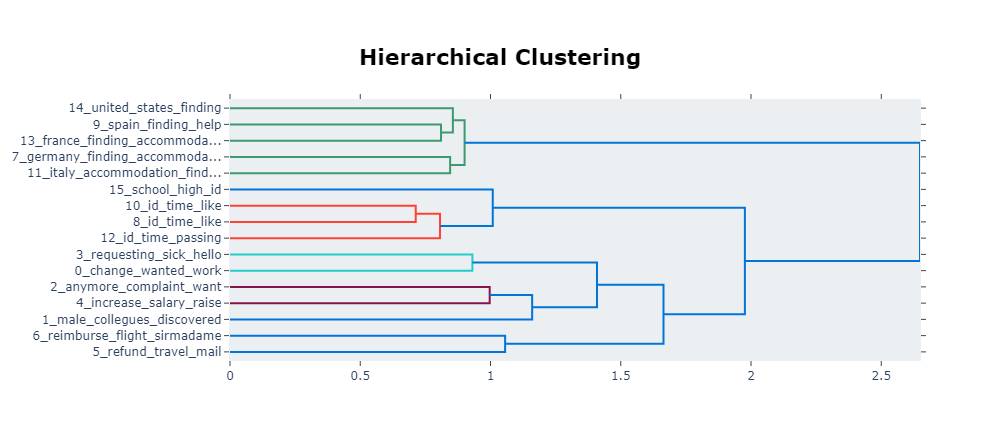
\includegraphics[width=\textwidth]{images/hierarchy_topic_model.png}
    \caption{Hierarchy of all topics generated by BERTopic}
    \label{fig:hierarchical_topicmodel}
\end{figure}


\begin{figure}[h] 
    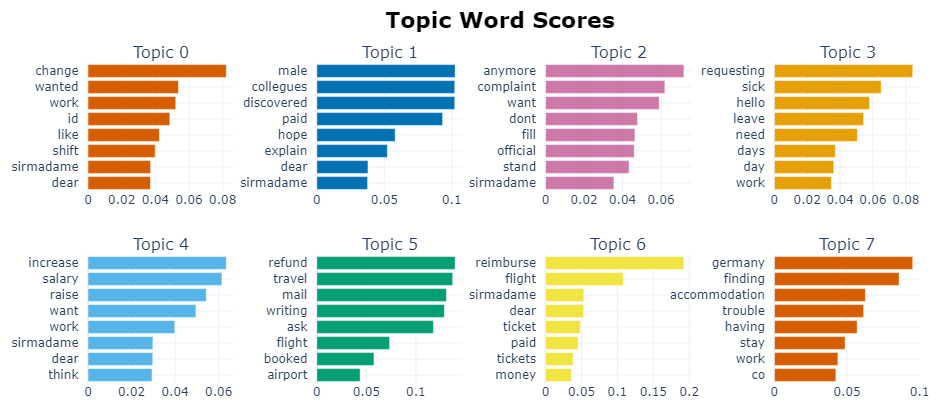
\includegraphics[width=\textwidth]{images/barchart_topicmodel.png}
    \caption{Main 8 topics generated by BERTopic}
    \label{fig:barchart_topicmodel}
\end{figure}    

\section{Additional Experiments}
\label{sec:additional_experiments}

In this section, we are going to describe various methods we have tried for the generation of tickets which have not been included in the final version of the ticket generation for different reasons. \\
Some of these reasons are lack of computational power, not good enough results and lack of time. \\

\subsection{Topical Generation}
Zandie et al.\cite{zandie2021topical} have presented topical language generation, which consists of generating text conditioned on a specific chosen topic. The topic can be chosen by the users from a predetermined list of topics. The topics are represented as a distribution over a vocabulary, and they are extracted from a corpus using algorithms of Topic Modeling. \\
The algorithm used is Latent Semantic Analysis, which gives us scores for each token per topic. LSA is able to discover latent topics in a document-term matrix by utilizing Singular Value Decomposition (SVD) to decompose the matrix. \\
The topics are inferred to the text generation by adding the embedding of the topic to the logits of the model before the last softmax layer, where the parameter $\gamma$ control the topic inference ( the higher the parameter $\gamma$ is, the more the text generated will be about the topic chosen)
\begin{equation*}
    \begin{split}
        & P(t_j|\;x_i): \text{probability of topic j given word k} \\
        & S(x_i|\;x_{<i}): \text{logits of token i} \\
    \end{split}    
\end{equation*}

They used a threshold to increase the probability of only the tokens that already have a minimum probability to be sampled.
\begin{equation*}
        logprob(i) = 
        \begin{cases}
            logP(t_j|\;x_i),& \text{if } S(x_i|\;x<i)\geq \text{threshold}\\
            0,              & \text{otherwise}
        \end{cases}
\end{equation*}

The final equation is:
\begin{equation*}
    P(x_i|\;x{<i},t_j) = softmax(S(x_i|\;x_{<i}) + \gamma\;logprob(i))
\end{equation*}
\\
We experimented this method to generate the tickets' texts. The topic-word matrix was calculated starting from 20 Newsgroups, a dataset of 18000 news posts on 20 topics. \\

Topic used: football
\begin{adjustwidth}{1cm}{}
    [\dots] \\
    Ticket category: Life event\\
    Ticket sub-category: Health issues\\
    Date start absence: 24/08/2016\\
    Reason absence: a physiotherapy visit\\
    Subject: Request for sick leave for 1 day\\\\
    Dear Sir/Madame, my name is Adriana Giulietti. I am requesting football medical treatment on the following dates : - 28 nfl season 2016 (from 30th of August regular football game) professional training session in Milan from 29 football football league match between FC Portcullis football conference matches and other 
\end{adjustwidth}

Topic used: president, government
\begin{adjustwidth}{1cm}{}
    [\dots] \\
    Ticket category: Life event\\
    Ticket sub-category: Health issues\\
    Date start absence: 25/12/2012\\
    Reason absence: Hordeolum\\
    Subject: Request for sick leave for 2 days\\\\
    Dear Sir/Madame, my name is Cristian Manso. I am requesting sick pay or vacation from you because state government has decided to cancel the contract which was signed on 20 th of 
    December 2012 with head office called president and deputy leader states house republic functions as a general administration department in charge common services like public works system
    \end{adjustwidth}

    

The possible future implementations of the ticket generation could be completely executed with a unique prompt, letting the user choose the topic from a set of pre-trained topics. This would be more flexible than the current method since to add new categories it would be sufficient to add a new row to the topic-word matrix. \\
However, the current results were not satisfying: the created tickets were not fluent and we did not find a corpus to create a topic-word matrix of topics related to the HR ticketing environment.

\subsection{Fine-tune GPT}
GPT can be adapted to a particular task by fine-tuning, either by supplying it with a dataset tailored to said task, or by manually adjusting the model's parameters. This process allows the model to be customized and to achieve much better results on the desired task. \\
As mentioned before, we want to generate tickets with a language and style similar to emails. Fine-tuning the model on the \textit{Enron dataset} should improve the performance of the model at generating new Enron-style emails compared to the generic trained model. \\
We tried fine-tuning GPT-J on only the \textit{\_sent\_mail} folders of the dataset. However, the tickets generated were not much different than the ones created by the base model. The evaluation was carried out only by looking at the tickets generated one by one, without using any sort of metrics.\\
After various tests, we ascertained that with prompt tuning we could have equal results as with the fine-tuning of the model, avoiding to spend time to fine-tune the model.

\chapter{Use Cases}
\label{sec:Use_Cases}

In order to assess the suitability of the HR ticket dataset for downstream machine learning applications in HR, we exploit the obtained dataset using as labels the categories of the tickets. \\
The goal of testing different downstream machine learning tasks on the dataset is to show that our dataset is sufficiently rich to enable meaningful learning. \\
All the experiments have been carried out using as training data the dataset generated by the model, whereas the test data used was the tickets collected with the survey. \\ 
One of the main motivations to acquire the survey tickets was to have data that had no biases, or at least biases different from ours. Using a portion of the HR tickets dataset as test data would be meaningless, since the model would not necessarily be tested with data that was outside of the one it had been trained with. On the contrary, achieving good results on a portion of the HR ticket dataset would assert the performance of the models used and not the usefulness of the dataset.

\section{Classification}
Sentence classification is a natural language processing task that involves assigning a predefined category or label to a given sentence. One way to approach sentence classification is to use word embeddings, which are numerical representations of words that capture their meaning and context within a sentence. Word embeddings can be generated using various techniques, such as training a neural network on a large dataset of text or using a pre-trained language model. \\
Once the word embeddings have been generated, you can input them into a classifier along with other features of the sentence, such as its grammatical structure, to make predictions about the sentence's category or label. The classifier uses the word embeddings as input to make predictions about the sentence's category or label. \\
We used two different pre-trained language models: BERT and fastText. We chose BERT because it is a widely used and well-studied model, and our objective was not to find the absolute best classifier, but only to show that the dataset could be used as training data. \\
Instead, we chose fastText to have an option that was CPU-friendly, and that could be trained in a matter of a few minutes. \\
The training data used were the texts of the 16000 tickets that compose the HR ticket dataset, whereas the test data were the survey tickets. The labels were the combination of ticket category and ticket subcategory of each ticket ( Ex. "Life event\_Health issues").


\subsection{FastText Classifier}
FastText is a library developed by Facebook AI Research that provides a set of training algorithms for supervised learning of word embeddings from raw text and also can be used to build and train supervised text classification models. \\
FastText creates word embeddings using a combination of character n-grams and word n-grams. To do this, fastText first breaks each word in the training text into its constituent character n-grams. For example, the word "cat" might be broken into the character n-grams "c", "ca", "cat", "a", "at", and "t". These character n-grams are then used to generate vectors. The word embeddings are calculated as the sum of their n-gram vectors. \\
To learn the embeddings of these n-grams, fastText uses a skip-gram model, which is a type of model that maximizes the probability of observing a word given its context, or in other words its surrounding words. By using this approach, fastText is able to learn high-quality word embeddings that capture the syntactic and semantic information of words. \\
The fastText classification uses the fastText embeddings as input to the model, and in particular:
\begin{algorithm}
    \caption*{fastText Classification}
    \begin{algorithmic}[1]
      \State Words representation are averaged into a text representation
      \State The text representation is fed to a linear classifier
      \State The output of the linear classifier is given as input to a softmax function to compute the probability distribution over a set of predefined classes
    \end{algorithmic}
\end{algorithm}


\subsection{BERT classifier}
BERT (Bidirectional Encoder Representation from Transformers) is a model developed by Google AI based on the transformers architecture. BERT was trained on a large corpus on two different tasks: Masked Language Modeling and Next Sentence Prediction. \\
Through the use of MLM, in the training phase, 15\% of the tokens in a sentence are obscured and BERT can then be utilized to utilize the surrounding words in both directions to predict the masked tokens, facilitating bidirectional learning from the text. \\
On the other hand, NSP helps the model understand the relationships between sentences. Specifically, in the training phase, 50\% of the examples are actually successive sentences, while in the other 50\% of the cases this condition is not respected. \\
BERT is quite straightforward to fine-tune, we just need to plug in the necessary layers at the top of the BERT architecture and fine-tune for a sufficient number of epochs the model end-to-end. \\
The first token of a BERT embedding is the [CLS] token, which is a special token that acts as an aggregate representation of the sentence. The final embedding of the [CLS] token is used as input for the classification task. The most simple method, which is also the method used by the BERTForSequenceClassification class by HuggingFace, is to take the embedding of the [CLS] token at the last hidden layer and fed it to a single layer of a feed-forward network. The layer of the feed-forward network will have n input, where n is the dimension of the embedding of a token, and m output, where m is the desired number of outputs. \\
The final model is shown in \autoref{fig:bert_class}
\begin{figure}[h] 
  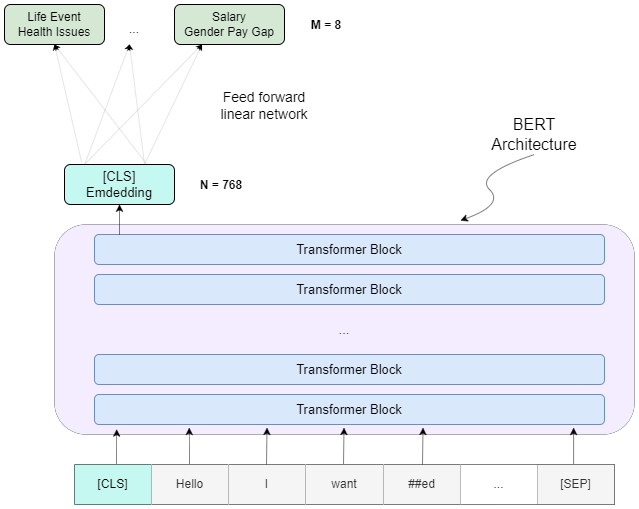
\includegraphics[width=\textwidth]{images/bert_class.drawio.png}
  \caption{Schema of BERT classification}
  \label{fig:bert_class}
\end{figure}

\subsection{Results}
In this section we show the results of the classification experiments. We want to reiterate that the point of the experiments was not to get the best possible results, therefore the models were not trained for a large number of epochs and we did not try an excessive number of possible hyperparameters.
The hyperparameters tried are shown in \autoref{table:hyp_fasttext} and \autoref{table:hyp_bert}. If a hyperparameter is not shown in the table it means we have used its default value. \\
The technique used for finding the optimal hyperparameters is Grid Search, which means we have trained and tested the models for each combination of all the chosen values of the hyperparameters to determine the hyperparameters' set which achieves the best results.

\begin{table}[h]
  \begin{tabular}{|l|l|}
  \hline
  Size of context window (ws)                   & 5      \\ \hline
  epochs                                        & 20     \\ \hline
  minimal number of word occurrences (minCount) & 1      \\ \hline
  max length of word ngram (wordNgrams)         & 3      \\ \hline
  learning rate (lr)                            & 0.5    \\ \hline
  learning update rate (lrUpdateRate)           & 100    \\ \hline
  sampling threshold (t)                        & 0.0001 \\ \hline
  \end{tabular}
  \caption{Hyperparameters fastText}\label{table:hyp_fasttext}
\end{table}

\begin{table}[h]
  \begin{tabular}{|l|l|}
  \hline
  epochs           & {[}3, 5{]}                              \\ \hline
  learning rate    & {[}1e-05, 5e-04, 1e-04, 5e-05, 5e-06{]} \\ \hline
  weight decay     & {[}0.001, 0.01, 0.05{]}                 \\ \hline
  train batch size & {[}8, 16{]}                             \\ \hline
  warmup steps     & 500                                     \\ \hline
  \end{tabular}
  \caption{Hyperparameters BERT}\label{table:hyp_bert}
  \end{table}

%TODO: add results
As we expected, fastText performs worse than BERT, achieving an $f_1$ score of only 0.41. \\
On the other hand, the BERT classifier with hyperparameters\begin{itemize}
  \item epochs: 5
  \item learning rate: 5e-05
  \item weight decay: 0.001
  \item train batch size: 8
  \item warmup steps: 500
\end{itemize}
achieved an $f_1$ score of 0.78. We show also the confusion matrix( \autoref{fig:conf_matrix_bert_class} ) to highlight how the majority of errors come from two sub-categories that belong to the same category, in particular, "Gender wage gap"-"Salary raise" and "Personal issues"-"Health issues". In some way, this validates our initial decision on the taxonomy of the tickets.
\begin{figure}[h] 
  \centering
  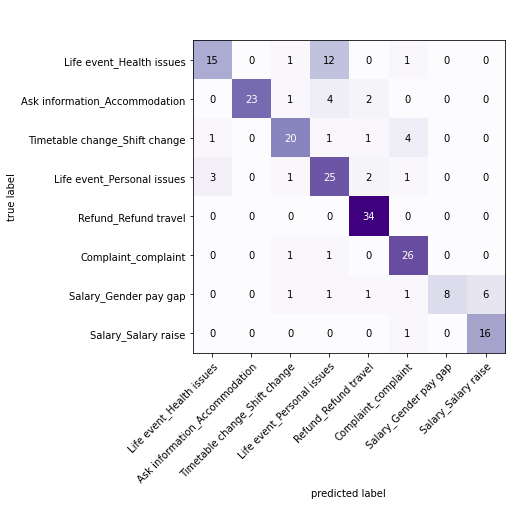
\includegraphics[width=0.8\textwidth]{images/conf_matrix_bert_class.png}
  \caption{Confusion matrix of Ticket classification with BERT}
  \label{fig:conf_matrix_bert_class}
\end{figure}    

\section{Anonymization}

Anonymization of personal data refers to the process of removing personally identifiable information (PII) from data sets so that the individuals represented in the data cannot be identified. This is accomplished by either completely removing or replacing identifiable data with generic values. The purpose of anonymization is to protect the privacy of individuals while still allowing the data to be used for legitimate purposes. \\
Most of the recent implementations of anonymization work by masking the personal information of a person, such as names and surnames, telephone numbers, addresses, credit card numbers and so on. \\
One of the most famous libraries for anonymization is Presidio, developed by Microsoft. Presidio exploits pattern recognition with regex and Named Entity Recognition to find all the personal information and mask them. \\
The main disadvantage of such techniques is that often the personal subject can be identified through the so-called quasi-identifiers, that more often than not are not masked.
\\Here reported some examples that are not masked by Presidio:\\ \\
Original sentence
\begin{adjustwidth}{1cm}{}
    The new intern at my office, the one with red hair, caught covid last week 
\end{adjustwidth}
Sentence redacted by Presidio
\begin{adjustwidth}{1cm}{}
    The new intern at my office, the one with red hair, caught covid \textless DATE\_TIME \textgreater
\end{adjustwidth}
Original sentence
\begin{adjustwidth}{1cm}{}
    The boss of the HR department has made some weird comments about how I dress
\end{adjustwidth}
Sentence redacted by Presidio
\begin{adjustwidth}{1cm}{}
    The boss of the HR department has made some weird comments about how I dress 
\end{adjustwidth}
Our new approach exploits a Sequence to Sequence model called T5
T5 is a model released by Google in 2019, it is a standard encoder-decoder transformer that, unlike BERT, always returns strings as outputs. This is why it is called a sequence-to-sequence model. \\
T5 is a unified model that can be applied for many downstream tasks, such as sentiment analysis, sentence completation, question answering\dots\\
In T5 architecture there are \textit{adapted layers} after each feed-forward layer, whose scope is to diminish the number of parameter updates for each fine-tuned model. In fact, \textit{adapted layers} are dense-ReLU-dense blocks that are designed so that their input dimensionality and output dimensionality are equal. This lets us insert them into the Transformer architecture without other changes. When fine-tuning for each different task, only the \textit{adapted layers} and the normalization layers will be updated. This results in a considerable reduction of parameter updates.\\
We followed a few-shot learning approach with T5. Rather than relying on a large amount of training data to allow a pre-trained model to adjust to a given task accurately, few-shot learning employs the use of a few examples to direct the training of a machine learning model with very minimal data. \\
For each category of tickets, we wrote 10 examples of "anonymized" tickets, where we removed all personal information and information that could be retraced to the original writer, maintaining only information that could be useful for analysis purposes.
Here are a couple of examples:\\ \\
Original sentence:
\begin{adjustwidth}{1cm}{}
    Dear Sir/Madame, I cannot stand anymore this discrimination and prejudice against French people at work
\end{adjustwidth}
Anonymization used for few-shot learning:
\begin{adjustwidth}{1cm}{}
    The employee is filling a complaint for discrimination based on nationality 
\end{adjustwidth}
Original sentence:
\begin{adjustwidth}{1cm}{}
    Hello, my name is Zacaredas Pinilla and I work at Laguna-Franco Spain. I am having trouble finding accommodation in the Algeciras area so if you could help me with this matter it would be greatly appreciated
\end{adjustwidth}
Anonymization used for few-shot learning:
\begin{adjustwidth}{1cm}{}
    The employee is asking for help finding an accommodation
\end{adjustwidth}
\begin{figure}[h] 
    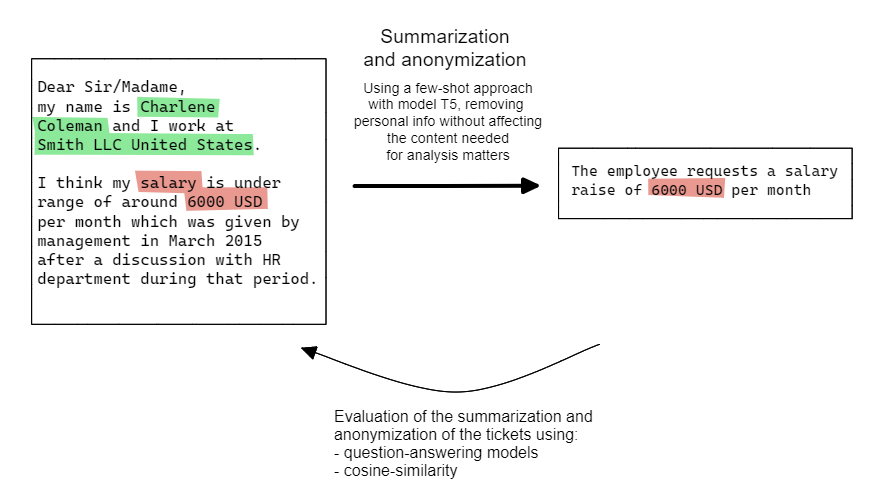
\includegraphics[width=\textwidth]{images/ticket_anonymization_schema.png}
    \caption{Schema of Ticket Anonymization}
    \label{fig:schema_ticket_anonymization}
\end{figure}    
To evaluate the goodness of anonymization and how much of the information has remained after the anonymization we have used three different methods:
\begin{itemize}
    \item \textbf{QAGS}: Questions Answering and Generation for summarization
    \item \textbf{SUMMAQA}: Unsupervised metric for reinforced summarization model 
    \item \textbf{Cosine Similarity}
\end{itemize}  
These models were created originally to evaluate the goodness of a summarization, we have adapted them to be used for evaluating our anonymization. \\
The first two methods follow the same philosophy: they generate questions to ask both the original version and the anonymized version of the tickets, looking if the answers are coherent. We call them Questions and Answers models.
However they have few key differences. SummaQA do not create natural sentence questions but uses as questions the masked version of the sentences. Instead QAGS create natural language questions using a pre-trained model.
\subsection*{QAGS}
QAGS is an automatic evaluation protocol that is based on the assumption that if we reply to questions considering as factual bases the summary and the source, we can determine if the summary/anonymization is consistent with its source by comparing the answers. \\
QAGS works like this:
\begin{algorithm}
    \caption*{QAGS}
    \begin{algorithmic}[1]
      \State A BART model is fine-tuned for question generation: the model receives both the answers and the source article from the NewsQA dataset and is trained to maximize the likelihood of the paired question
      \State At test time, named entities and noun phrases are extracted from the context using spaCy and are considered as answers candidates. The summary is used as the context.
      \State The BART model generates question based on the summary and its entities
      \State A BERT model is fine-tuned for Question Answering on the SQuAD dataset
      \State We answer with the help of the fine-tuned BERT model the questions generated beforehand using both the source article and the summary to get two sets of answers. 
      \State We compare the corresponding answers using an answer similarity metric, and we get a final score averaging the answer similarity metric (f1 score) over all questions
    \end{algorithmic}
\end{algorithm}

\subsection*{SUMMAQA}
SUMMAQA works similarly to QAGS, the main difference is that there is not a generative model to create the questions, in particular:
\begin{algorithm}
    \caption*{SUMMAQA}
    \begin{algorithmic}[1]
      \State We find all the entities in the source text (the original ticket) with Spacy
      \State Create one sentence (which will be our question) for each entity. We keep only the sentence in which the entity is if there are more sentences. The entity will be masked. Ex: "Yesterday I went to Paris" becomes "Yesterday I went to [MASK]"
      \State The MASKED entities will be the True labels when calculating the metrics
      \State We answer to the questions generated before using a fine-tuned version of BERT model, using both the source and the summarization/anonymization as contexts
      \State We compare the answers and calculate the f1 score for both contexts
    \end{algorithmic}
\end{algorithm}
\subsection*{Cosine Similarity}
We measured the cosine similarity between sentence embeddings of original text and summarization. The sentence embeddings used were calculated using Sentence-BERT, a modified version of the pretrained BERT network that uses siamese networks to obtain more meaningful embedding of the sentence, compared to getting the embedding of the [CLS] token or to average all the other emeddings.

%TODO: maybe put little schema of Siamese network of sentence-bert

\begin{figure}[h] 
    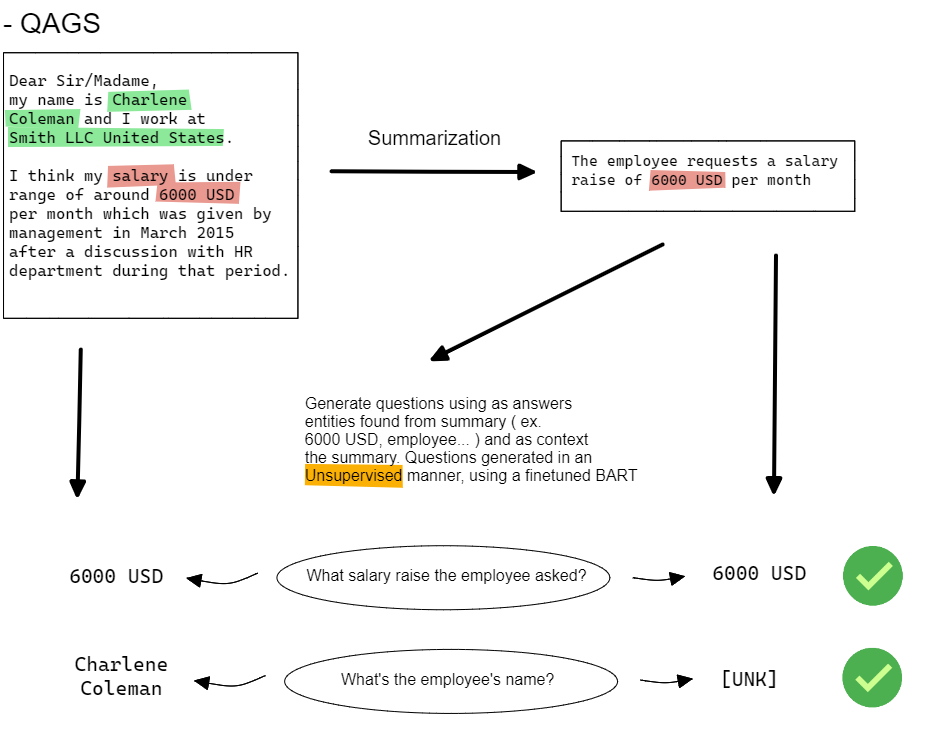
\includegraphics[width=\textwidth]{images/qa_models_qags.png}
    \caption{Schema of QAGS}
    \label{fig:schema_qags}
\end{figure}    

\begin{figure}[h] 
    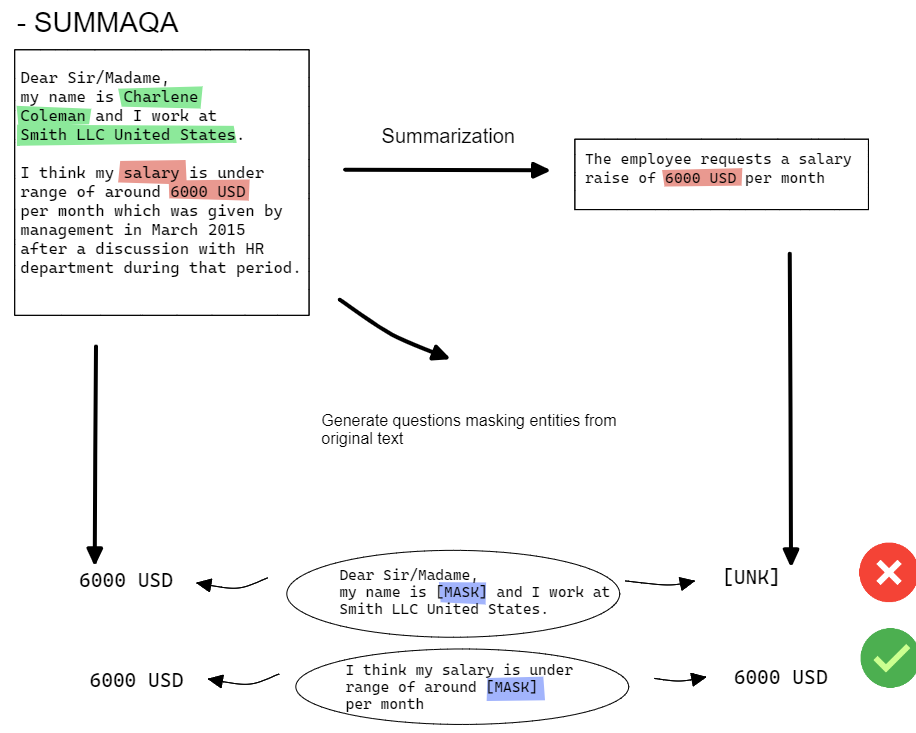
\includegraphics[width=\textwidth]{images/qa_models_summaqa.png}
    \caption{Schema of SUMMAQA}
    \label{fig:schema_summa_qa}
\end{figure}    

\begin{figure}[h] 
    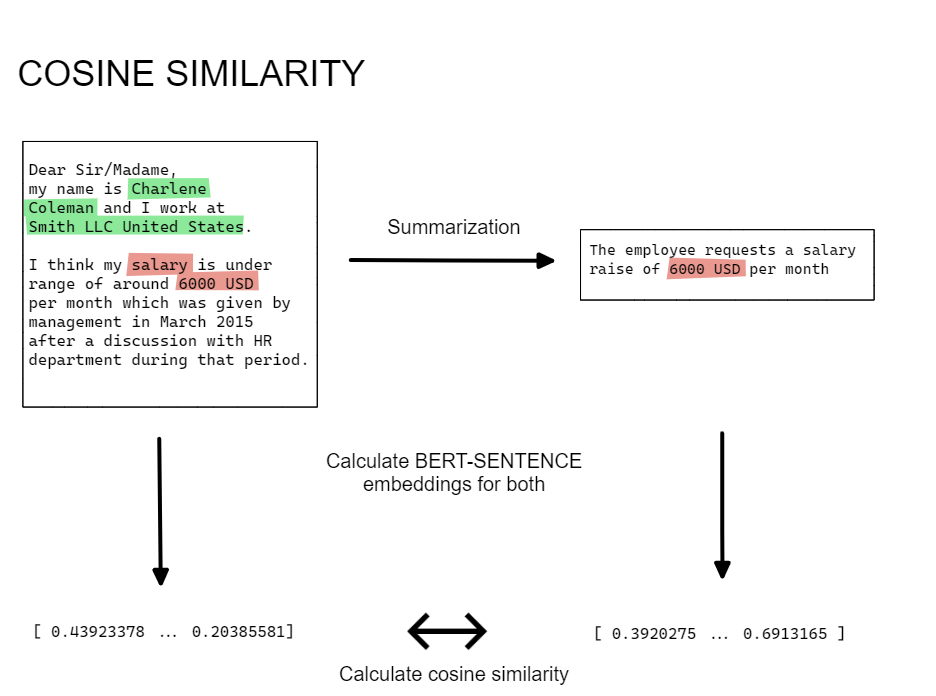
\includegraphics[width=\textwidth]{images/cosine_similarity.png}
    \caption{Schema of Cosine Similarity for }
    \label{fig:schema_cosine_similarity}
\end{figure}    





\clearpage
\section{Named Entity Recognition}
\label{sec:ner}
Named entity recognition is the process of automatically identifying and classifying named entities in a text. This can include identifying and categorizing named entities such as people, organizations, locations, and so on. \\
NER systems might be used to automatically extract information from a large collection of documents, such as identifying all mentions of specific named entities or analyzing the relationships between different named entities. \\

\subsection{Weak labeling}
During the creation of the ticket, we tried to automatically save also the entities of the ticket. With entities, we do not mean the classical entities used for NER, but the original variables specific to a ticket's category (complete list in \autoref{table:categoriesTable}). \\
Finding the entities in the prompt is trivial, since the positions are fixed in the template, and the filling operation is managed by us. \\
Example:
\begin{adjustwidth}{1cm}{}
    From: \$\{email\} \\
    To: \$\{company email\} \\
    First name: \$\{first name\}\\
    Last name: \$\{last name\}\\
    Company: \$\{company\}\\
    Date: \$\{ticket date\}
    Date start absence: \colorbox{yellow!30}{\$\{date\_start\_absence\}}\\
    Reason absence: \colorbox{yellow!30}{\$\{reason\_absence\}}\\
    Subject: Request for sick leave for \colorbox{yellow!30}{\$\{days\}}    
\end{adjustwidth}
Though the template and prompt serve as our starting point to generate the actual ticket text, it is only this latter part that would be present in a real ticket. Identifying the locations of the entities is not straightforward since I usually provide only the initial information and a limited template, with the rest of the generation being done by GPT. \\
Once the ticket is generated, to find the entities in the generated text I use 2 different approaches:
\begin{itemize}
    \item Exact match
    \item Heuristics
\end{itemize}
The exact match is straight-forward, it just looks for the exact same words in the generated text, and if the word/words are found, the entity is added to the list of entities of the ticket
However this method often does not work, since GPT could use only part of the entity ( Ex: "A medical consultation" is in the text as "a consultation") or slightly alter the entity ( ex: 01/10/1998 $\rightarrow$ the first of October of 1998 ) \\
This is the reason why we implemented manually a set of different rules to find modified versions of the original entity in the text. These versions do not cover every possible case, since they are hard-coded by us from experience and by looking at how GPT behaves, this is why we called this approach "Heuristics". \\
Some of these heuristics are:
\begin{itemize}
    \item Check not only the full entity, but also subsets of it removing stopwords\\
    Example: \\
    reason\_of\_absence: "An Urinary Tract Infection" $\rightarrow$
                 \begin{itemize}
                    \item "Urinary Tract Infection"
                    \item "Urinary Tract"
                    \item "Tract Infection"
                    \item "Urinary"
                    \item "Tract"
                    \item "Infection"
                \end{itemize}
    \item Check all the possible version of a percentage text\\
    "5\%", "5 \%", "5.0\%", "5 percent", \dots
    \item Check different formats of date\\
    MM/DD/YYYY, DD/MM/YYYY, "First of October", "1st of October", \dots

\end{itemize}
With this method, we were able to identify entities in only 6272 tickets out of the total 16000 tickets. The complete list of all the entities found is shown in \autoref{table:entities_found_heuristics}.

\begin{table}[h]
    \centering
    \begin{tabular}{|l|l|l|l|}
    \hline
    duration                 & 1016 & increase\_in\_percentage & 539 \\ \hline
    location                 & 1411 & work\_title & 33 \\ \hline
    date                     & 70   & wage\_gap & 421 \\ \hline
    work\_shift              & 70   & number\_of\_days & 982 \\ \hline
    reason\_of\_change       & 7    & date\_start\_absence & 3 \\ \hline
    to\_who                  & 1221 & description\_life\_event & 1214 \\ \hline
    reason                   & 1119 & date\_travel & 112 \\ \hline
    complaint                & 106  & airport & 28 \\ \hline
    salary                   & 376  & & \\ \hline
    \end{tabular}
    \caption{Entities found with heuristics}\label{table:entities_found_heuristics}
\end{table}

\subsection{Classical NER}
\label{sec:classical_ner}
Token classification is a common technique used in NER to identify and classify named entities in a text. In token classification, the text is first divided into individual tokens, which are typically words or phrases. The model then predicts a label for each token, indicating the type of named entity it represents.\\
To assign the labels to the tokens we used the BIO(Beginning, Inside, Outside) format, where the B tag is used for the first token of an entity, the I tag for the rest of the tokens of the entity and lastly the O tag is used for the tokens that do not belong to any entities. \\
Example:
\begin{adjustwidth}{1cm}{}
    Alex B-PER\\
    is O\\
    going O\\
    to O\\
    Los B-LOC\\
    Angeles I-LOC\\
    in O\\
    California B-LOC
\end{adjustwidth}
The labels assigned to each token are then used for a token classification task, using a RoBERTa model and the Spacy training pipeline. \\
We used the default Spacy parameters for the training. \\
The survey tickets, used as always as our test set, were manually labeled by ourselves. \\
%TODO: maye put image of schema token classification for NER
The results were not satisfying, we achieved a $f_1$ score of 0.34 on the exact matching and a $f_1$ score of 0.45 on the partial matching. When the model finds the correct entity for all the tokens and only the tokens of an entity, it's considered an exact matching. Whereas, when the model finds the correct entity for only a subset of the token of an entity, then is considered a partial match\\
Example exact match:
\begin{adjustwidth}{1cm}{}
    to O\\
    Los LOC\\
    Angeles LOC\\
    in O\\
\end{adjustwidth}
Example partial match:
\begin{adjustwidth}{1cm}{}
    to O\\
    Los LOC\\
    Angeles O\\
    in O\\
\end{adjustwidth}
The main problem we encountered was that the NER model was not able to recognize the different entities of the same type depending on the context. For example, the model could not recognize the difference between a date of start absence ( entity of request of time off due to health reasons) and a date of travel ( entity of request of refund for travel).

\subsection{Our approach to NER}
\label{sec:ner_nc}
To overcome the limits of the first approach, we developed a new approach based on transfer learning and sentence classification. \\
The main intuition behind the new approach is to use the pre-trained spacy NER model and exploit the entities found by the base model to extract our entities. \\
First of all, we build a dictionary of the matchings between entities of Spacy and our entities. We decided to work on a subset of our entities and not consider all the entities that did not have a clear matching with Spacy entities. In \autoref{table:entities_match} we show all the matchings. 
\begin{table}[h]    
    \resizebox{\textwidth}{!}{
    \setlength\extrarowheight{18pt}
    \begin{tabular}{|l|l|}
    \hline
    Category                       & Entities matching                                              \\ \hline
    Ask information\_Accommodation & \shortstack[l]{\{"location": "GPE", \\"duration": "DATE"\}}                       \\ \hline
    Life event\_Health issues      & \shortstack[l]{\{"date\_start\_absence": "DATE", \\"number\_of\_days": "DATE"\}} \\ \hline
    Refund\_Refund travel          & \shortstack[l]{\{"date\_travel": "DATE",\\ "location": "GPE"\}}                  \\ \hline
    Salary\_Gender pay gap         & \{"wage\_gap": "PERCENT"\}                                     \\ \hline
    Salary\_Salary raise           & \shortstack[l]{\{"increase\_in\_percentage": "PERCENT",\\"salary": "MONEY"\}}    \\ \hline
    Timetable change\_Shift change & \{"date": "DATE"\}                                             \\ \hline
    \end{tabular}}
    \caption{Matching of our entities with Spacy entities}\label{table:entities_match}
\end{table}
Then, we scan our dataset and look, for all categories, the entities shown in \autoref{table:entities_match}. If we find an entity not present in the table, it is filtered out. For each entity, we will have an array of the type [ ENTITY, START\_CHAR, END\_CHAR ] (\autoref{fig:ticket_NER_NC_1}).\\
\begin{figure}[h] 
    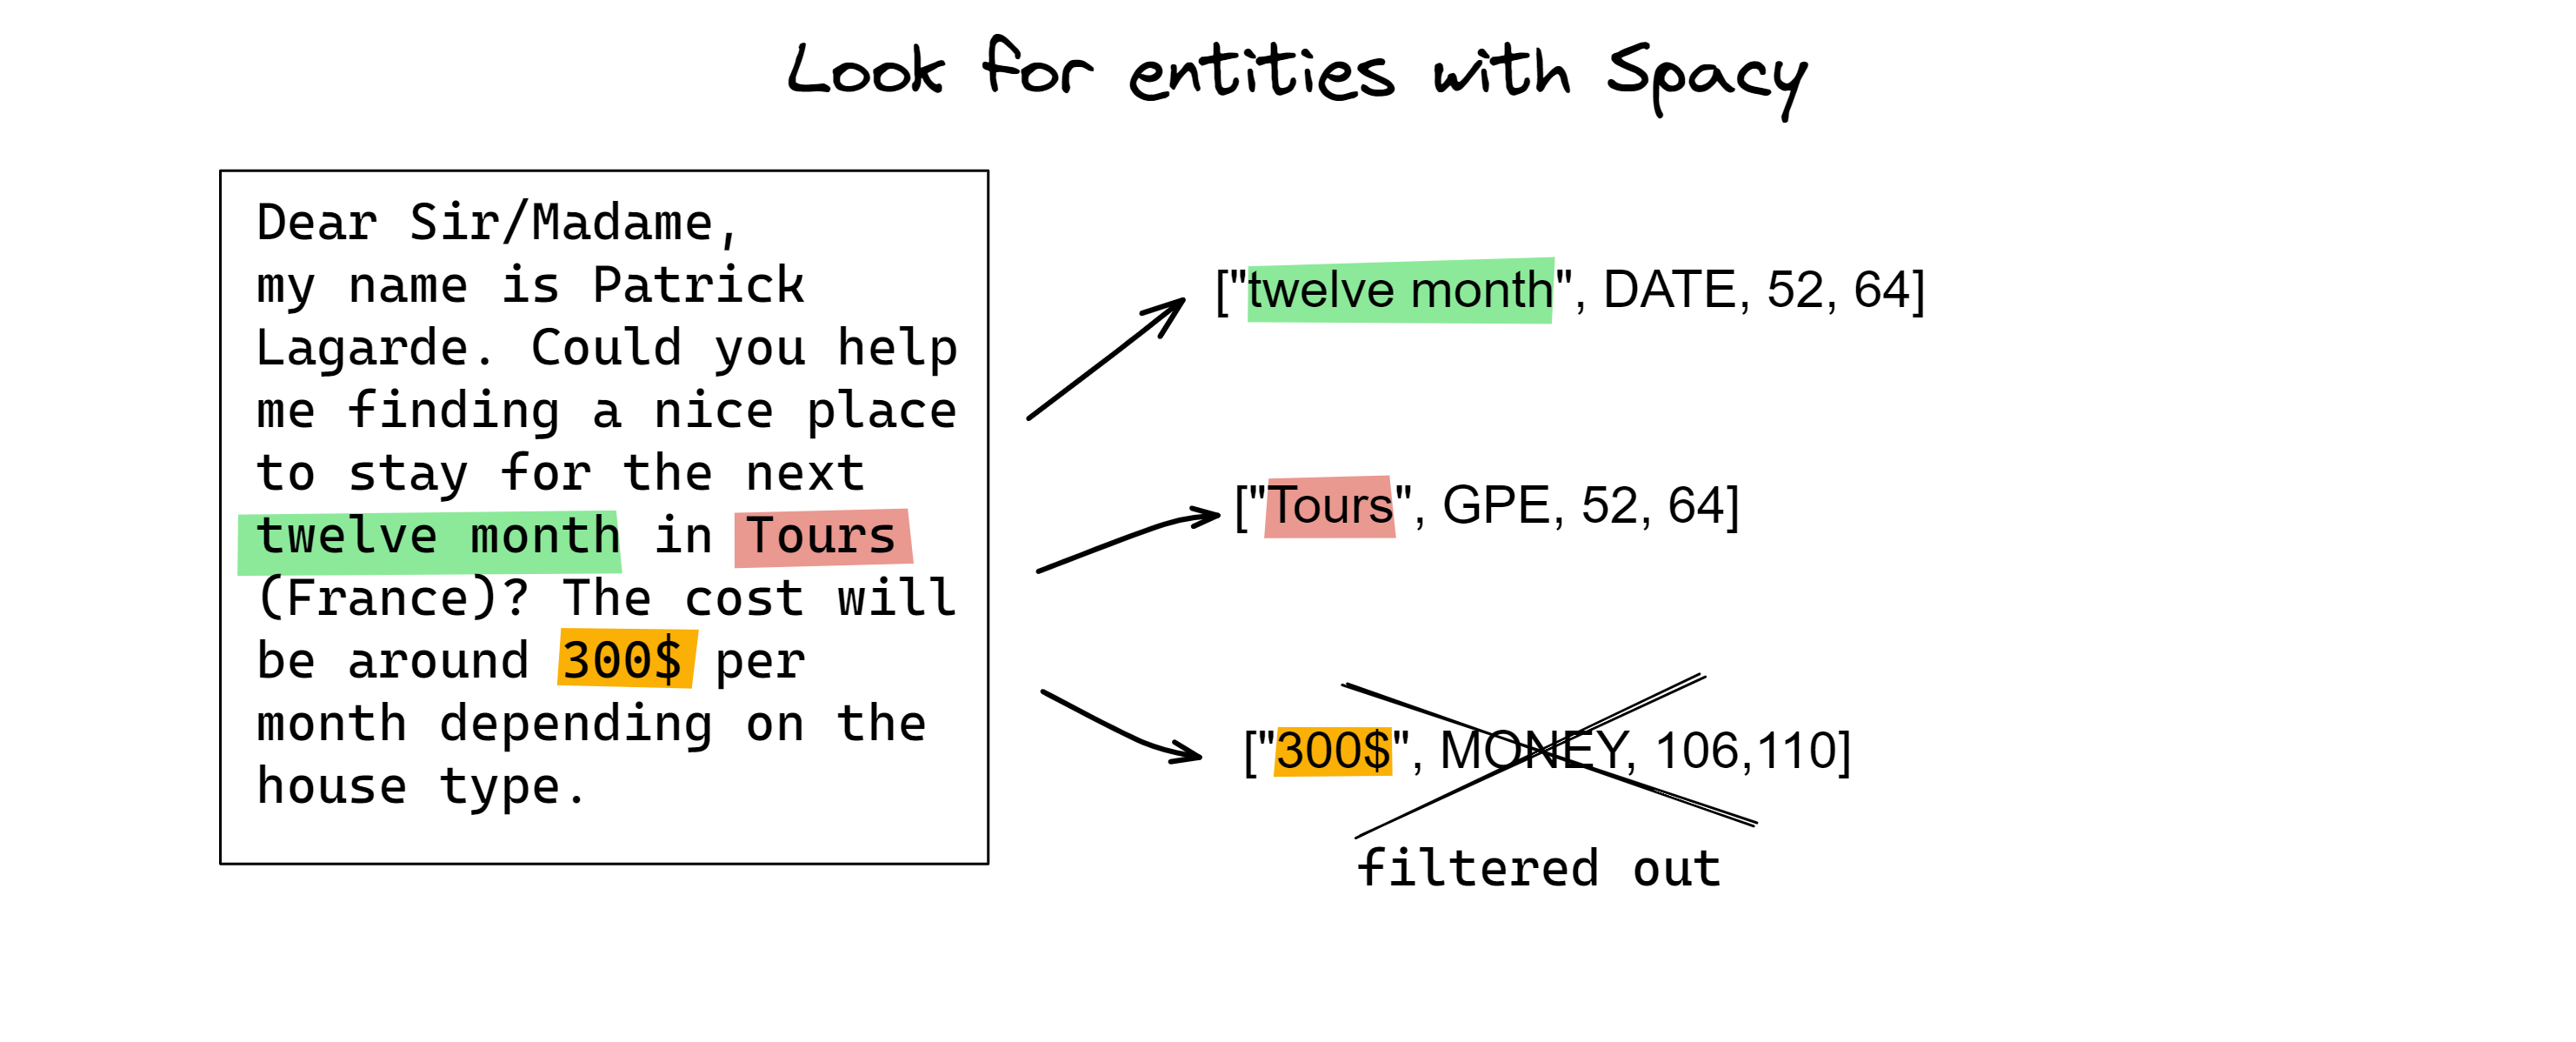
\includegraphics[width=\textwidth]{images/NER_nc_1.png}
    \caption{Ticket NER preprocessing part 1}
    \label{fig:ticket_NER_NC_1}
\end{figure}    
After that, we tokenize the text of all the tickets and we look up for each ticket its entities' tokens. Then for each entity, we save the indexes of the corresponding tokens, so for example if the entity "twelve months" is split into two tokens "twelve" and "month", which are the $22^{nd}$ and $23^{rd}$ tokens of the text, then we will save ["twelve months", DATE, [22,23]]. \\
We also had to manage the case in which a token is not present in the tokenizer vocabulary, so is split into sub-tokens. We took advantage of the fact that if a word is split into two or more words the new tokens will have the prefix "\#\#". \\
The number of tokens for each entity can vary, for practical reasons in the training phase we set the maximum number of tokens to $N=50$ (\autoref{fig:ticket_NER_NC_2}).
\begin{figure}[h] 
    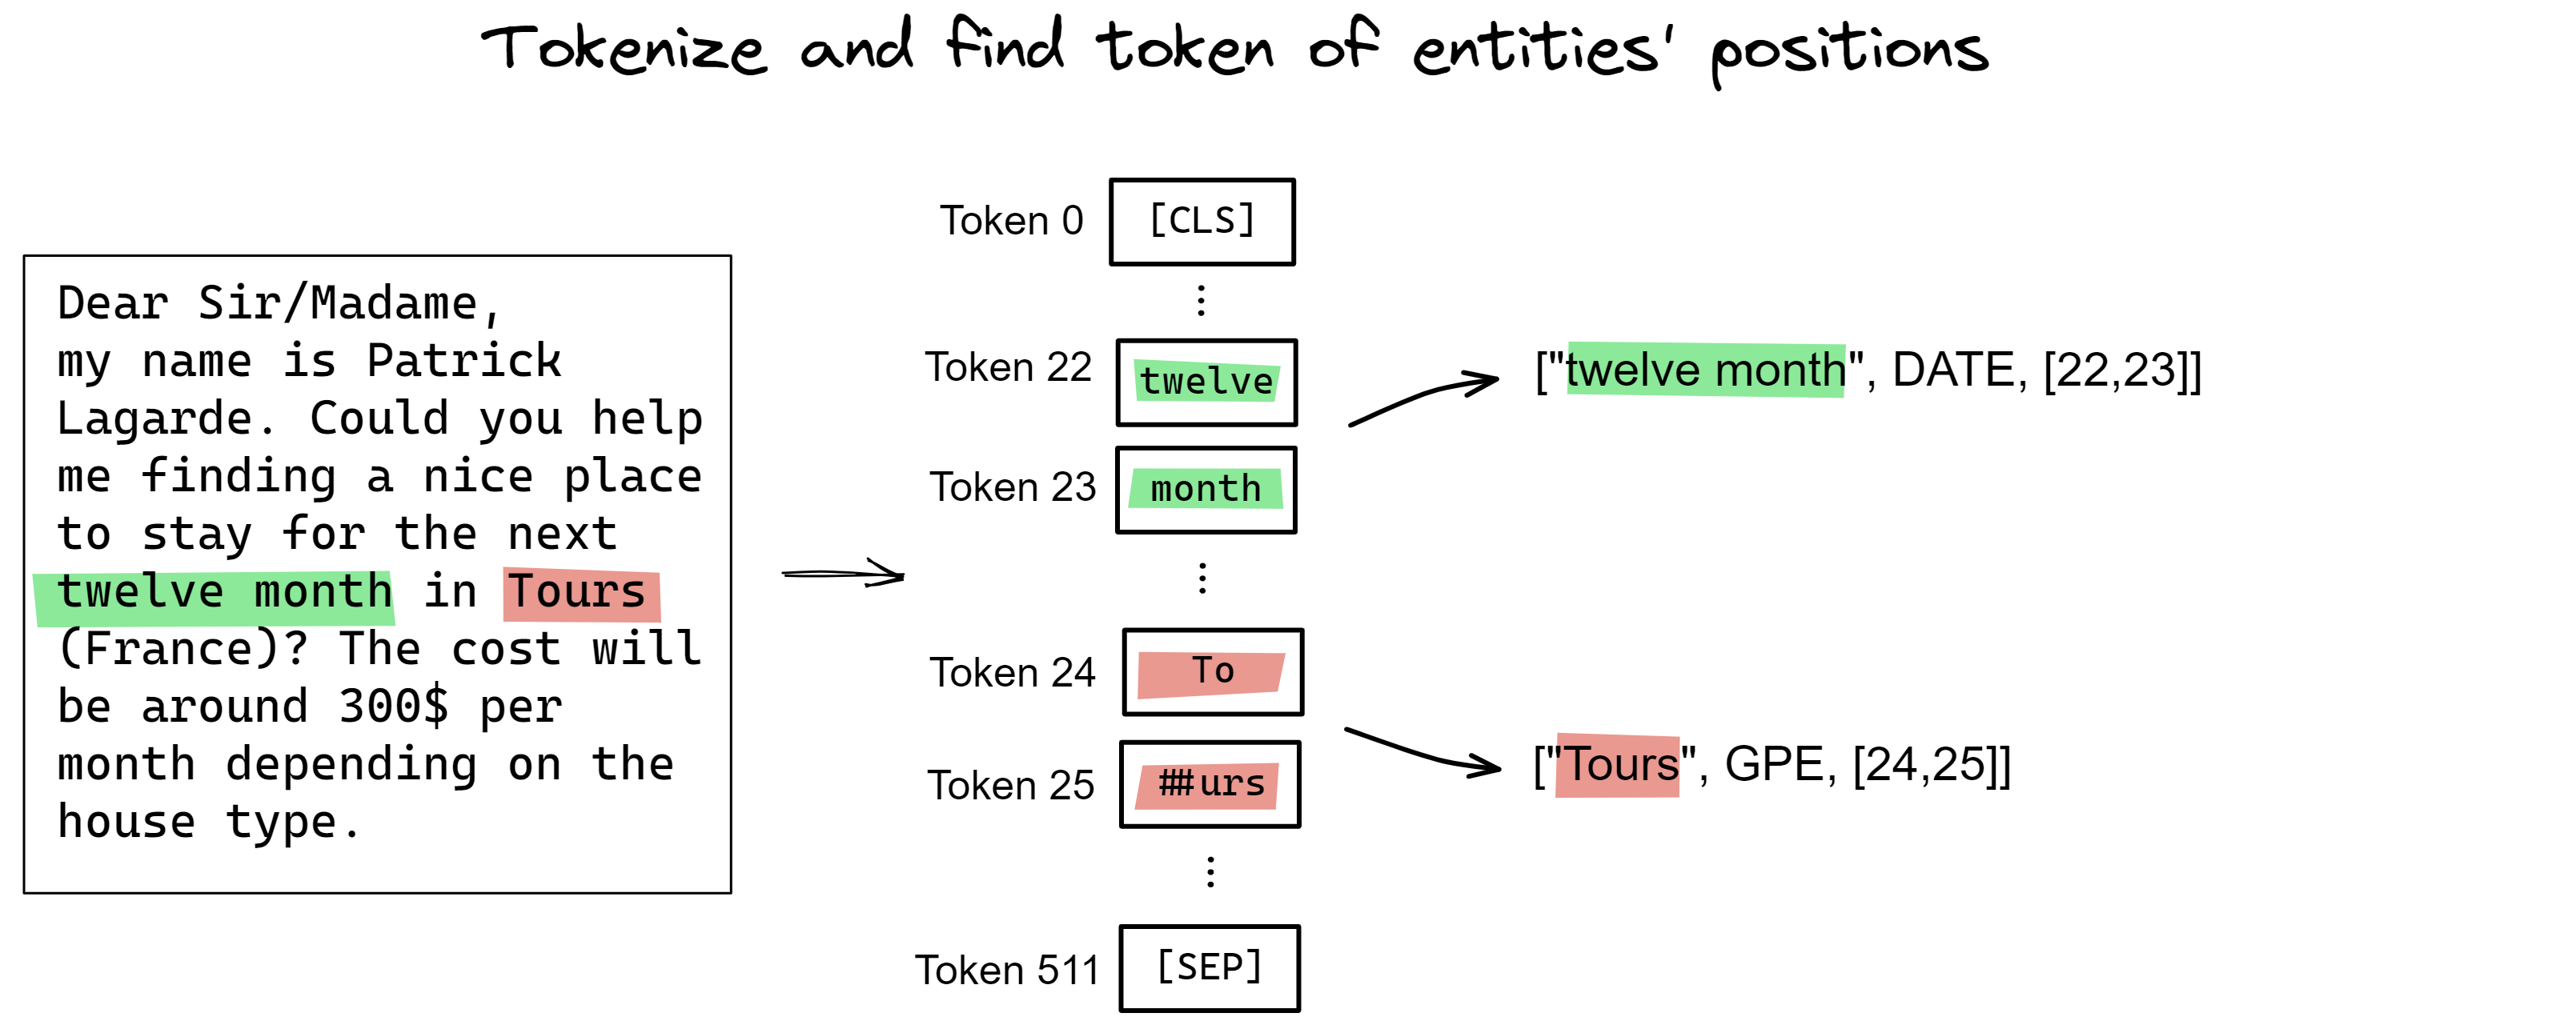
\includegraphics[width=\textwidth]{images/NER_nc_2.png}
    \caption{Ticket NER preprocessing part 2}
    \label{fig:ticket_NER_NC_2}
\end{figure}    
Now we have all we need for the training. The base architecture is a \textit{bert-base-cased} model, which we modified on the last layer. \\
In the training phase, we pass to the BERT model at each step the tickets' texts and their entities with the indexes of the matching tokens. For each entity of the ticket, there will be a training record. The ticket will be unpacked into 512 tokens, and each token will be processed by the BERT architecture (same architecture as the classifier \autoref{fig:bert_class}). \\
At the last layer, instead of passing the [CLS] token to a classifier, we concatenate the [CLS] token with the average of all the embeddings of the tokens of the current entity. This is the reason why we preprocessed the dataset to find the indexes of the tokens' indexes for the entities. In BERT base each token has a dimension $d=768$, so the input of the last feed forward neural network will be $N=1536$. The output dimension will be $M=10$ (\autoref{fig:ticket_NER_NC_3}). The labels of the training are the combination of the ticket category and the entity, since for each entity found in a ticket we generate a record ( For example if there are 3 entities in a ticket, there will be 3 records in the training set with the same ticket text, but that will have a different token embedding for the classification in the last layer and they will have different labels)\\
\begin{figure}[h] 
    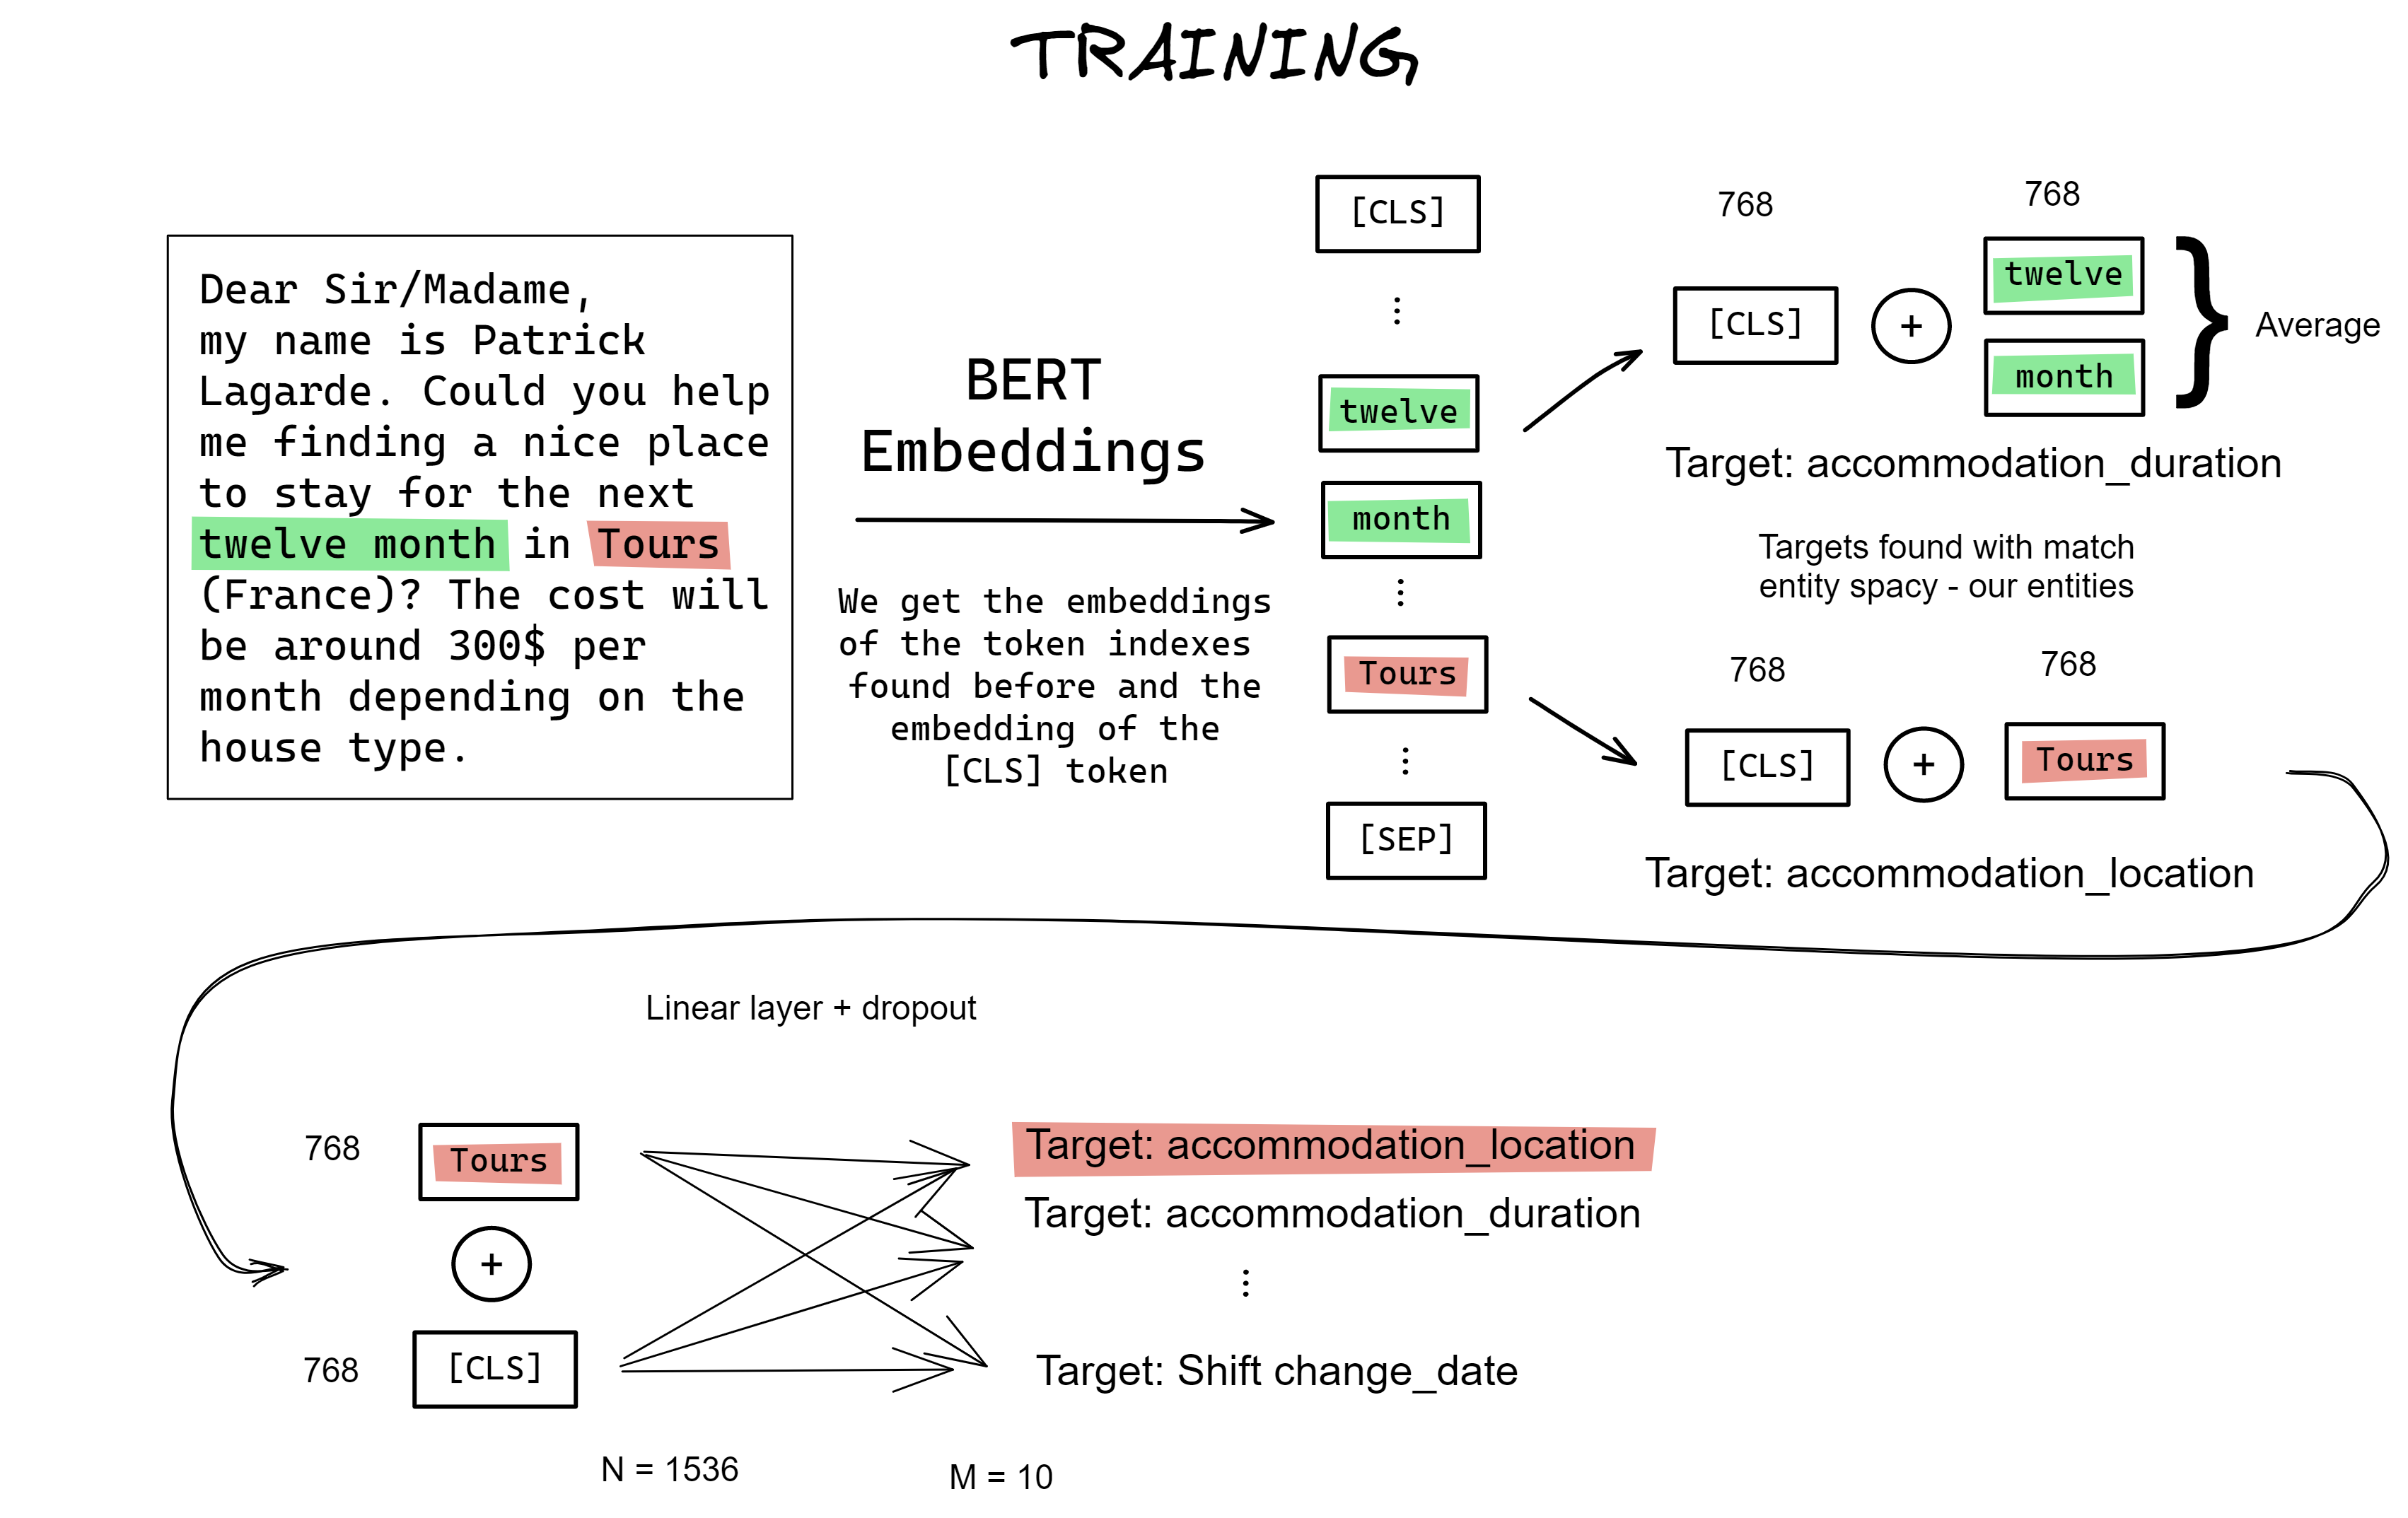
\includegraphics[width=\textwidth]{images/NER_nc_3.png}
    \caption{Ticket NER training}
    \label{fig:ticket_NER_NC_3}
\end{figure}
At test time, for each ticket in the test set, we analyze it with Spacy and we find all the entities. Then we filter the entities: we cannot filter based on the label, since at test time in theory we do not know the label of the tickets. Therefore we filter the entities based on the list of all entities used in all tickets' categories. \\
Then, as in the training phase, for each entity we build a new record composed of the output of the [CLS] token through the model architecture and of the average of the tokens' embeddings. \\
For each ticket in the test set we obtain a prediction of its category combined with the entity currently analyzed. 
\subsubsection*{Results}
We are able to achieve way better results with the new method that combines a ticket classifier with a NER model. On the test set we achieve a $f_1$ score of 0.96. \\
In \autoref{fig:ticket_NER_NC_conf_matrix} we show the confusion matrix of the classification. \\
We believe that we are able to achieve such good results because there are few entities that are shared between more categories, and the union of the information of the ticket ([CLS] token) and the information of the entity makes it easy for the model to distinguish both the category and the entity.
\begin{figure}[h] 
    \centering
    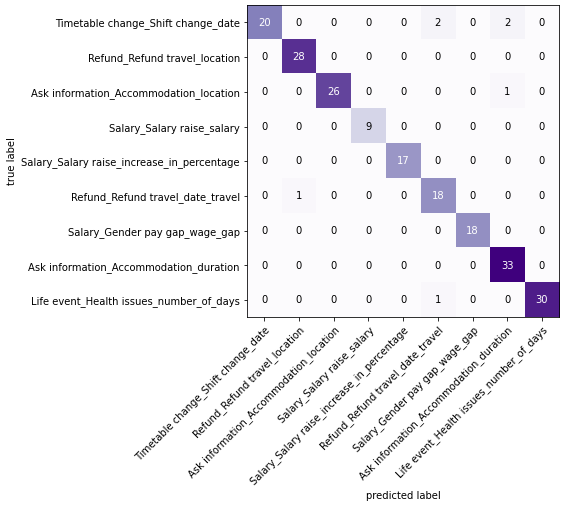
\includegraphics[width=0.8\textwidth]{images/conf_matrix_ner_nc.png}
    \caption{Ticket NER confusion matrix}
    \label{fig:ticket_NER_NC_conf_matrix}
\end{figure}   



\chapter{Conclusion}
\label{sec:conclusion}

Firstly, we developed a taxonomy of HR tickets and created a series of templates for each category. We discussed the considerations behind constructing the templates and then researched free-open datasets related to each category. We employed privacy-preserving techniques such as Bayesian Networks to process the datasets. \\
Then, we identified the state-of-the-art models for text generation, followed by a discussion of their respective novelties. After that, we discussed the generative model chosen by us, GPT-J, and the reasonings behind the decision. We explained in detail the theory behind Transformers and the novelties of GPT-J with respect to the other generative models. \\
We examined the model's ability to generate texts from two angles: we looked how the inputs influence the inputs and how each neuron of the model behaves scross different steps of the generation. \\
We conducted a survey in order to demonstrate that our dataset could resemble real tickets and that the tickets created by our application could be used to train machine learning models which worked also in real scenarios. \\
Specifically we tested the usefulness of the dataset on three different use cases: classification of tickets, anonymization of tickets and named entity recognition. \\
For the classification of tickets we trained and tested two different models. 
Whereas for the anonymization task, we used a novel approach that summerizes and rewrites the original text. Lastly, we experimented a classical named entity recognition model on our dataset and, after achieving not satisfying results, we developed a new technique that unifies a text classification task with named entity recognition.

We achieved good results on all three different tasks, therefore we can confidently state that the dataset we built could be used to train ML models for real-world applications. We recognize that each company has a distinct taxonomy for tickets, so we developed the \textit{Ticket Generator} application to facilitate the adaptation to different contexts.

% \paginavuota % it works even without stile=classica

\appendix
% \input{content/appendix/appendixA}

% \input{content/appendix/appendixB}

% endnotes here if needed

\phantom{0}
\cleardoublepage
\printbibliography[heading=bibintoc] % heading required to show it in ToC

\end{document}
